% \documentclass[sort&compress]{elsarticle}
% \documentclass[final,3p,times,onecolumn,sort&compress]{elsarticle}
% \documentclass[final,3p,times,twocolumn,sort&compress]{elsarticle}
\documentclass[review]{elsarticle}


\usepackage{lineno}
\modulolinenumbers[2]

\journal{Remote Sensing of Environment}

%% Packages
\PassOptionsToPackage{hyphens}{url}\usepackage{hyperref}
\usepackage{tabu}
\usepackage{booktabs}
\usepackage{breakurl}
\usepackage{float}
\usepackage{amsmath}
\usepackage{setspace}


%%%%%%%%%%%%%%%%%%%%%%%
%% Elsevier bibliography styles
%%%%%%%%%%%%%%%%%%%%%%%
%% To change the style, put a % in front of the second line of the current style and
%% remove the % from the second line of the style you would like to use.
%%%%%%%%%%%%%%%%%%%%%%%

%% Numbered
% \bibliographystyle{model1-num-names}

%% Numbered without titles
%\bibliographystyle{model1a-num-names}

%% Harvard
% \bibliographystyle{model2-names.bst}\biboptions{authoryear}

%% Vancouver numbered
% \usepackage{numcompress}\bibliographystyle{model3-num-names}

%% Vancouver name/year
% \usepackage{numcompress}\bibliographystyle{model4-names}\biboptions{authoryear}

%% APA style
%\bibliographystyle{model5-names}\biboptions{authoryear}

%% AMA style
% \usepackage{numcompress}
% \bibliographystyle{model6-num-names}

%% `Elsevier LaTeX' style
\bibliographystyle{elsarticle-num}

%%%%%%%%%%%%%%%%%%%%%%%

\begin{document}

\begin{frontmatter}

\title{Night and day: What is the influence and relative importance of urban characteristics on land surface temperature?}

%% or include affiliations in footnotes:
% \author[1]{T.M. Logan\corref{mycorrespondingauthor}}
% \cortext[mycorrespondingauthor]{Corresponding author}
% \ead[url]{www.tomlogan.co.nz}
% \ead{tom.logan@canterbury.ac.nz}

% \author[2]{B. Zaitchik}
% \author[3]{S. Guikema}
% \author[]{A. Nisbet}

% \address[1]{Civil and Natural Resources Engineering, University of Canterbury, New Zealand}
% \address[2]{Earth and Planetary Sciences, Johns Hopkins University, Baltimore, MD}
% \address[3]{Industrial and Operations Engineering, University of Michigan, Ann Arbor, MI}

\begin{abstract}
Heat waves are among the deadliest natural hazards and are expected to increase in frequency and severity under climate change. 
Their impacts in cities can be exacerbated by the urban heat island (UHI), but the mechanisms that underlie severity and timing of the UHI and its interactions with heat waves are poorly understood.
Understanding these mechanisms is necessary to design strategies that reduce land surface temperature and mitigate the effect of heat waves.
Making use of recently available high-resolution day and night thermal satellite imagery and employing advanced nonlinear statistical models, we seek to answer the question \textit{``What is the influence and relative importance of urban characteristics on land surface temperature, during both the day and night?''} 
To answer this question, we analyze urban land surface temperature in four cities across the United States.
In our analysis, we include variables related to vegetation, water, the built-environment, and topography. 
We model the effects of these variables using nonlinear statistical methods which allow for their independent effects to be assessed.
The effects from the daytime and nighttime analysis are compared to determine if previously reported relationships hold between cities and during both the day and night.
Our results suggest that vegetation and impervious surfaces are the most important urban characteristics associated with land surface temperature.
Increasing and decreasing these, respectively, is necessary for reducing high urban temperatures during both night and day.
Our results also demonstrate the potential for using nonlinear statistical analysis to investigate land surface temperature and its relationships with urban characteristics. 
For example, we can evaluate the compounding influence of two urban characteristics on the temperature.
Improved understanding of these relationships influencing both night and day land surface temperature will assist planners undertaking climate change adaptation and heat wave mitigation.
\end{abstract}

\begin{keyword}
LandSat; Land surface temperature; Urban canyon; Machine learning; Convolutional Neural Network
\end{keyword}

\end{frontmatter}

\linenumbers

\section{Introduction}
In a warming world, understanding the factors contributing to high land surface temperature (LST) and the urban heat island (UHI) will aid in adapting cities in mitigating urban heat for the health and wellbeing of their communities.
And mitigate they must; the 1995 Chicago heat wave, which killed more than 700 people,\footnote{The 2003 European heatwave killed 70,000 \cite{Robine2008-ky} and the 2015 European heat wave increased mortality up to 30\% \cite{Vicedo-Cabrera2016-si}} is expected to become an annual occurrence by 2080 \cite{klinenberg2015heat}. 
Heat waves' effect on people is exacerbated by the urban heat island (UHI) \cite{Wicki2017-fv, Echevarria_Icaza2016-fr}.
The UHI is understood to be a product of multiple factors including: enhanced absorption of solar radiation, geometric effects that limit radiative cooling and ventilation, anthropogenic heat from vehicles and buildings, air pollution that traps outgoing radiation, high ratios between sensible and latent heat flux due to low vegetation cover and high impervious land cover, and the radiative characteristics of building materials. % \cite{Oke2002-ta, Landsberg1981-mq, Rotach2005-yu}.
The result is increased diurnal and nocturnal temperatures that reduce people's ability to cool off, especially during the night, which drives an increase in mortality \cite{Echevarria_Icaza2016-fr, Murage2017-wj}.

Studies of urban heat include analyses of air temperature, which is a conventional meteorological variable that is often associated with health outcomes(e.g. \cite{Scott2016-lc}), and studies that use satellite-derived land surface temperature (LST) \cite{Imhoff2010-lf, Peng2012-iy, Peng2018-cp, Zhou2014-wc, Voogt2003-mm}.
LST correlates with air temperature at large scales, but there are differences at intra-urban scales \cite{Good2016-yk}.
While LST is not a conventional meteorological variable, it is directly related to the urban heat budget and has the advantage of being available with extensive spatial coverage in gridded satellite products \cite{Hung2006-qy}.
We analyze LST in this study.

Most existing LST studies focus on the daytime \cite{Peng2018-cp,Chun2018-so,Wang2019-water,Zhou2018-iy}.
However, the mechanisms and urban characteristics driving LST allegedly differ between night and day \cite{Hung2006-qy, Chun2017-mm, Nichol2005-mm, Wicki2017-fv, Echevarria_Icaza2016-fr,Sobstyl2018-wt, Peng2012-iy, Zhou2014-wc, Zhao2017-cc}. 
Given that UHI is primarily a nocturnal phenomena, the lack of study on nighttime LST leaves a critical gap in our understanding. 
This can now be addressed as high resolution nighttime satellite images have become available.

Most existing studies that have analyzed LST, particularly nighttime LST, have used low-resolution imagery, making it challenging to deduce a clear understanding of the influence and relative importance of the associated urban characteristics \cite{Chun2017-mm, Echevarria_Icaza2016-fr, Wicki2017-fv, Zhou2014-wc}. 
Additionally, these studies can be enhanced by: 1) studying multiple regions, 2) considering 2D and 3D urban characteristics, 3) diversifying their statistical models and relaxing their linear assumption, 4) rigorously testing and validating their models.
The data availability has limited previous nocturnal studies, meaning that many rely on MODIS images with a 1km resolution \cite{Zhou2014-wc, Echevarria_Icaza2016-fr,Wang2019-tree,Peng2012-iy}.
1km resolution makes it difficult to attribute LST to urban characteristics.
However, 100m resolution LandSat8 (L8) night scenes have recently become available. 
Due to the wide spatial availability of L8 imagery, comparative studies between cities that are necessary to understand the generalizability of findings \cite{Peng2012-iy, Hung2006-qy}, can now be conducted for day and night.

Existing studies have also been criticized for the explanatory variables they've used \cite{Chun2017-mm,Peng2018-cp}.
There is ongoing disagreement regarding the importance of 3D (e.g. building height) vs 2D (such as albedo) variables.  
Competing studies suggest that 3D factors are not important \cite{Berger2017-lx}, while others find that ignoring 3D incorrectly conflates the effect of different 2D variables \cite{Chun2017-mm}.
Beyond the 2D or 3D debate, important variables include green space, water bodies, albedo, and socio-economic factors \cite{Peng2018-cp}. 
However, many studies do not capture these categories and many analyze only the single effect of each variable \cite{Zhao2017-cc, Merbitz2012-xz, Unger2004-ry} (see \cite{Peng2018-cp, Chun2017-mm} for further discussion). 
Considering a variable in isolation, without accounting for potential conflating by other variables, limits the understanding of the interdependent effects that exist.

The third potential enhancement is in the statistical models.
Almost all studies use linear techniques (e.g. \cite{Li2017-yl, Peng2012-iy, Wicki2017-fv,Zhou2014-wc,Peng2018-cp,Echevarria_Icaza2016-fr,Chun2017-mm,Chun2018-so,Wang2019-tree,Wang2019-water}.
Using linear models incurs a number of major challenges that limit these studies' ability to explain the interdependencies between variables. 
The first is that many of the urban characteristics exhibit high multicollinearity \cite{Zhou2014-wc}.
The second is that linear models are limited in their ability to quantify the independent effects of characteristics and their relative influence on LST \cite{Peng2018-cp, Zhou2014-wc}.

Finally, most existing studies do not rigorously validate their models.
The approach they use to assess their accuracy is in-sample validation.
In-sample validation means that model accuracy is assessed with the same data used in the training, rather than unseen data. 
This risks overestimating the accuracy of their models.

The question we address is: \textit{``What is the influence and relative importance of urban characteristics on land surface temperature, during both the day and night?''}
To achieve this we conduct a comparative study of four cities in the United States using nonlinear statistical techniques which capture the interdependencies and relative importance between the urban characteristics.
In addressing our question, we will address the, at times fundamental, limitations of existing studies.
We look at nighttime temperature as well as daytime, we appropriately validate our statistical models, and we use tools that allow us to explore the interdependent, nonlinear, effects of urban characteristics on urban heat.
While we do not claim causality, understanding the associations between urban characteristics on temperatures can complement and further inform our understanding of the processes that lead to high urban land surface temperature.
The results therefore have implications for mitigating the severity of future heat waves.

\section{Data and Methods}
\subsection{Cities studied}

We study four cities in the contiguous United States (Figure \ref{fig:map}): Baltimore, MD; Detroit, MI; Phoenix, AZ; and Portland, OR. These four cities were selected as they include East and West coast cities, a mid-western city, and an arid central city. Phoenix, additionally, has been the subject of numerous other studies on land surface temperature. The cities were also selected due to lidar availability which is required for calculating the 3D variables. The constraint on selecting more cities was the time and computational requirements primarily for the LST and sky view factor calculations. 

Figure \ref{fig:map} shows the 500m gridded nighttime LST data for each of the cities and Figure \ref{fig:joy} shows the distribution of each city's 100m resolution day and night land surface temperature. 

\begin{figure*}
    \centering
    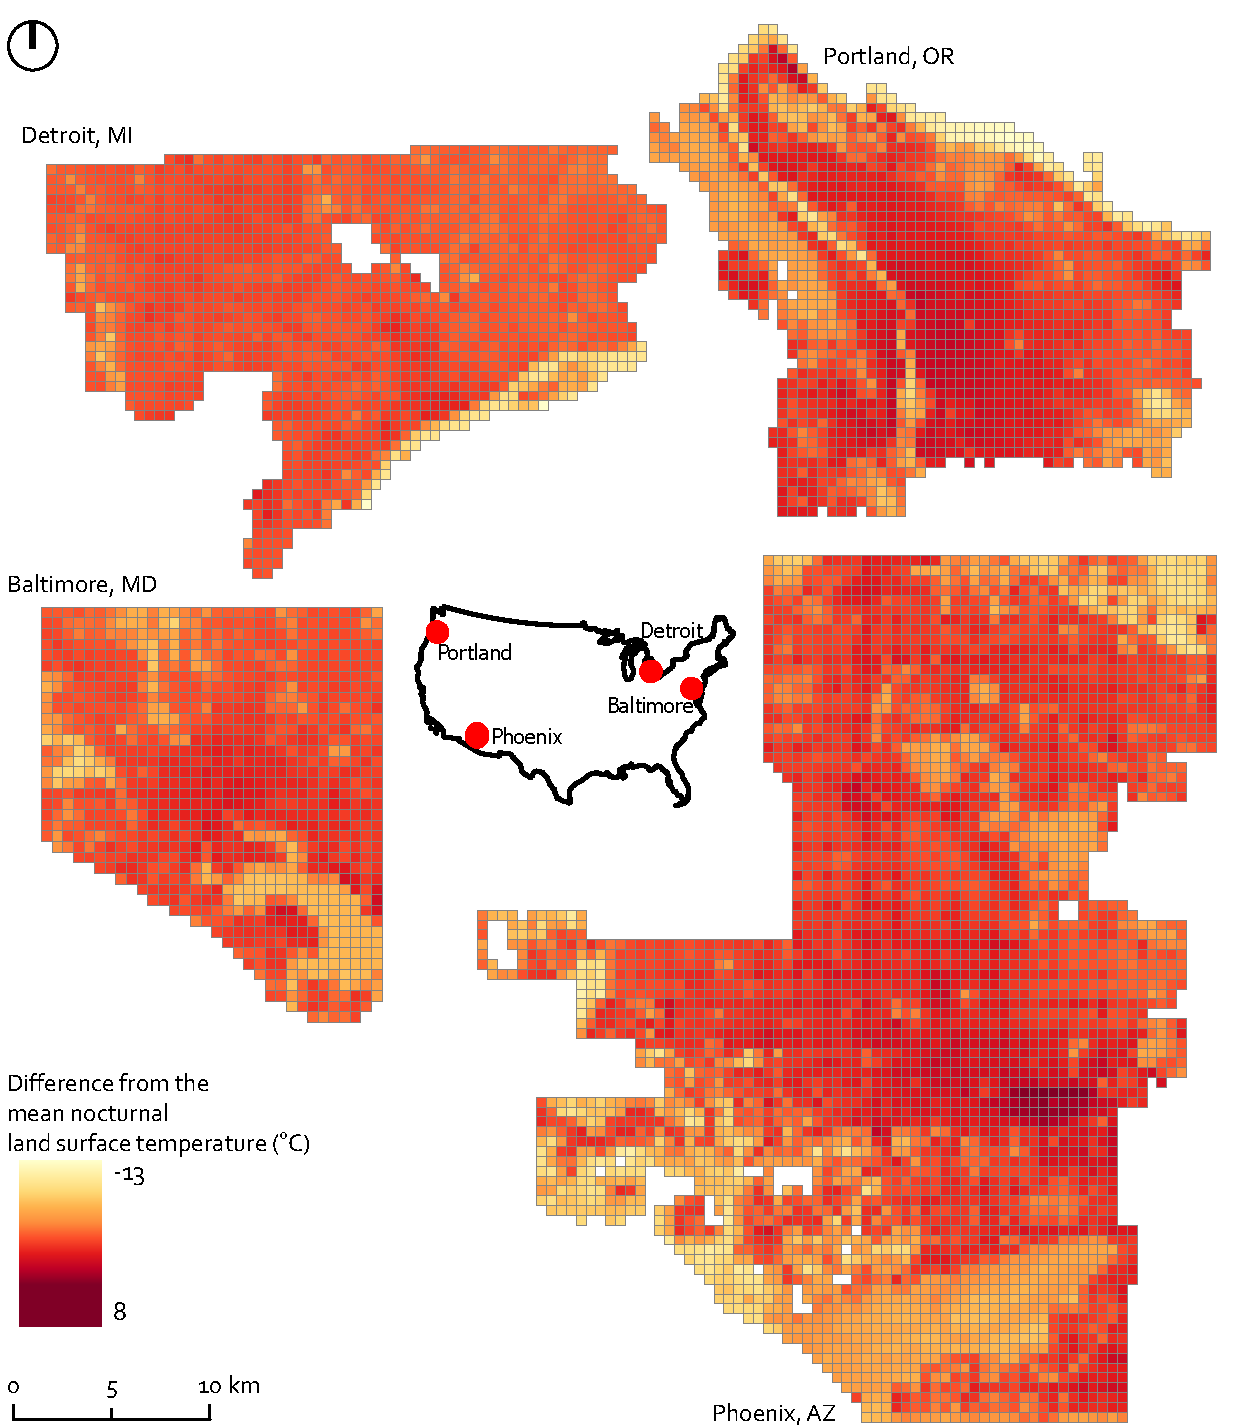
\includegraphics[width=\textwidth]{fig/report/map_nocturnal_lst.pdf}
    \caption[The nighttime land surface temperature in $^o$C, gridded into 500-meter cells, for the cities studied]{The nighttime land surface temperature in $^o$C, gridded into 500-meter cells, for the cities studied. This is change from the mean (average) for each city.}
    \label{fig:map}
\end{figure*}


\begin{figure}
    \centering
    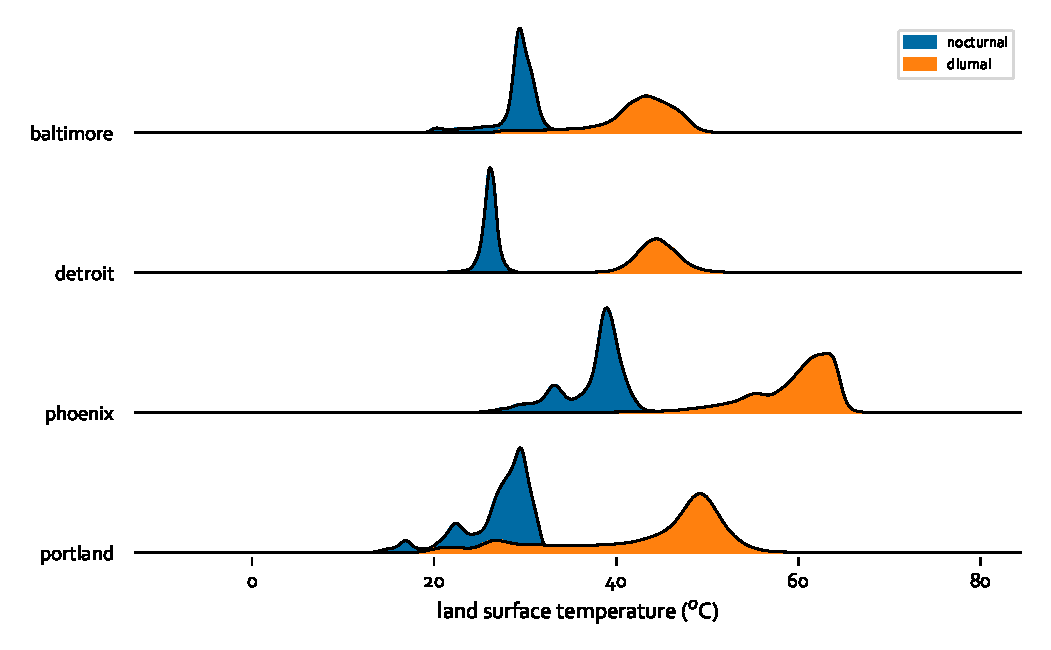
\includegraphics[width=\linewidth]{fig/report/joyplot_lst_100.pdf}
    \caption{The distribution of nocturnal and diurnal land surface temperature of the cities studied. 100m resolution.}
    \label{fig:joy}
\end{figure}

\subsection{Land surface temperature}
We calculate land surface temperature using Landsat 8 (Land Processes Distributed Active Archive Center product) imagery, land cover data, and an air temperature observation (data sources provided in \ref{tab:data}). 
Our code is available on our Github\footnote{URL redacted for review} repository, and is as follows:
We convert Band-10 digital-number data to top-of-atmosphere radiance \cite{Jimenez-Munoz2003-wc}. 
We correct for emissivity using land cover data \cite{Alipour2003-ym}, and then calculate the at-satellite brightness temperature \cite{Jimenez-Munoz2003-wc}. 
Finally, an atmospheric correction is made as per the mono-window algorithm \cite{Qin2001-jn} using the maximum observed temperature of the day from a nearby weather station. 
This follows the process is described in \cite{Scott2016-lc}. 

To ameliorate the effect of ephemeral changes \cite{Zhou2018-iy} we use at least three minimal-cloud images for each city and night/day period and calculate the mean of LST.

So we can conduct the comparative study between the cities, the land surface temperature for each city is calculated as the difference from the city's mean. 

\begin{figure}
    \begin{center}
    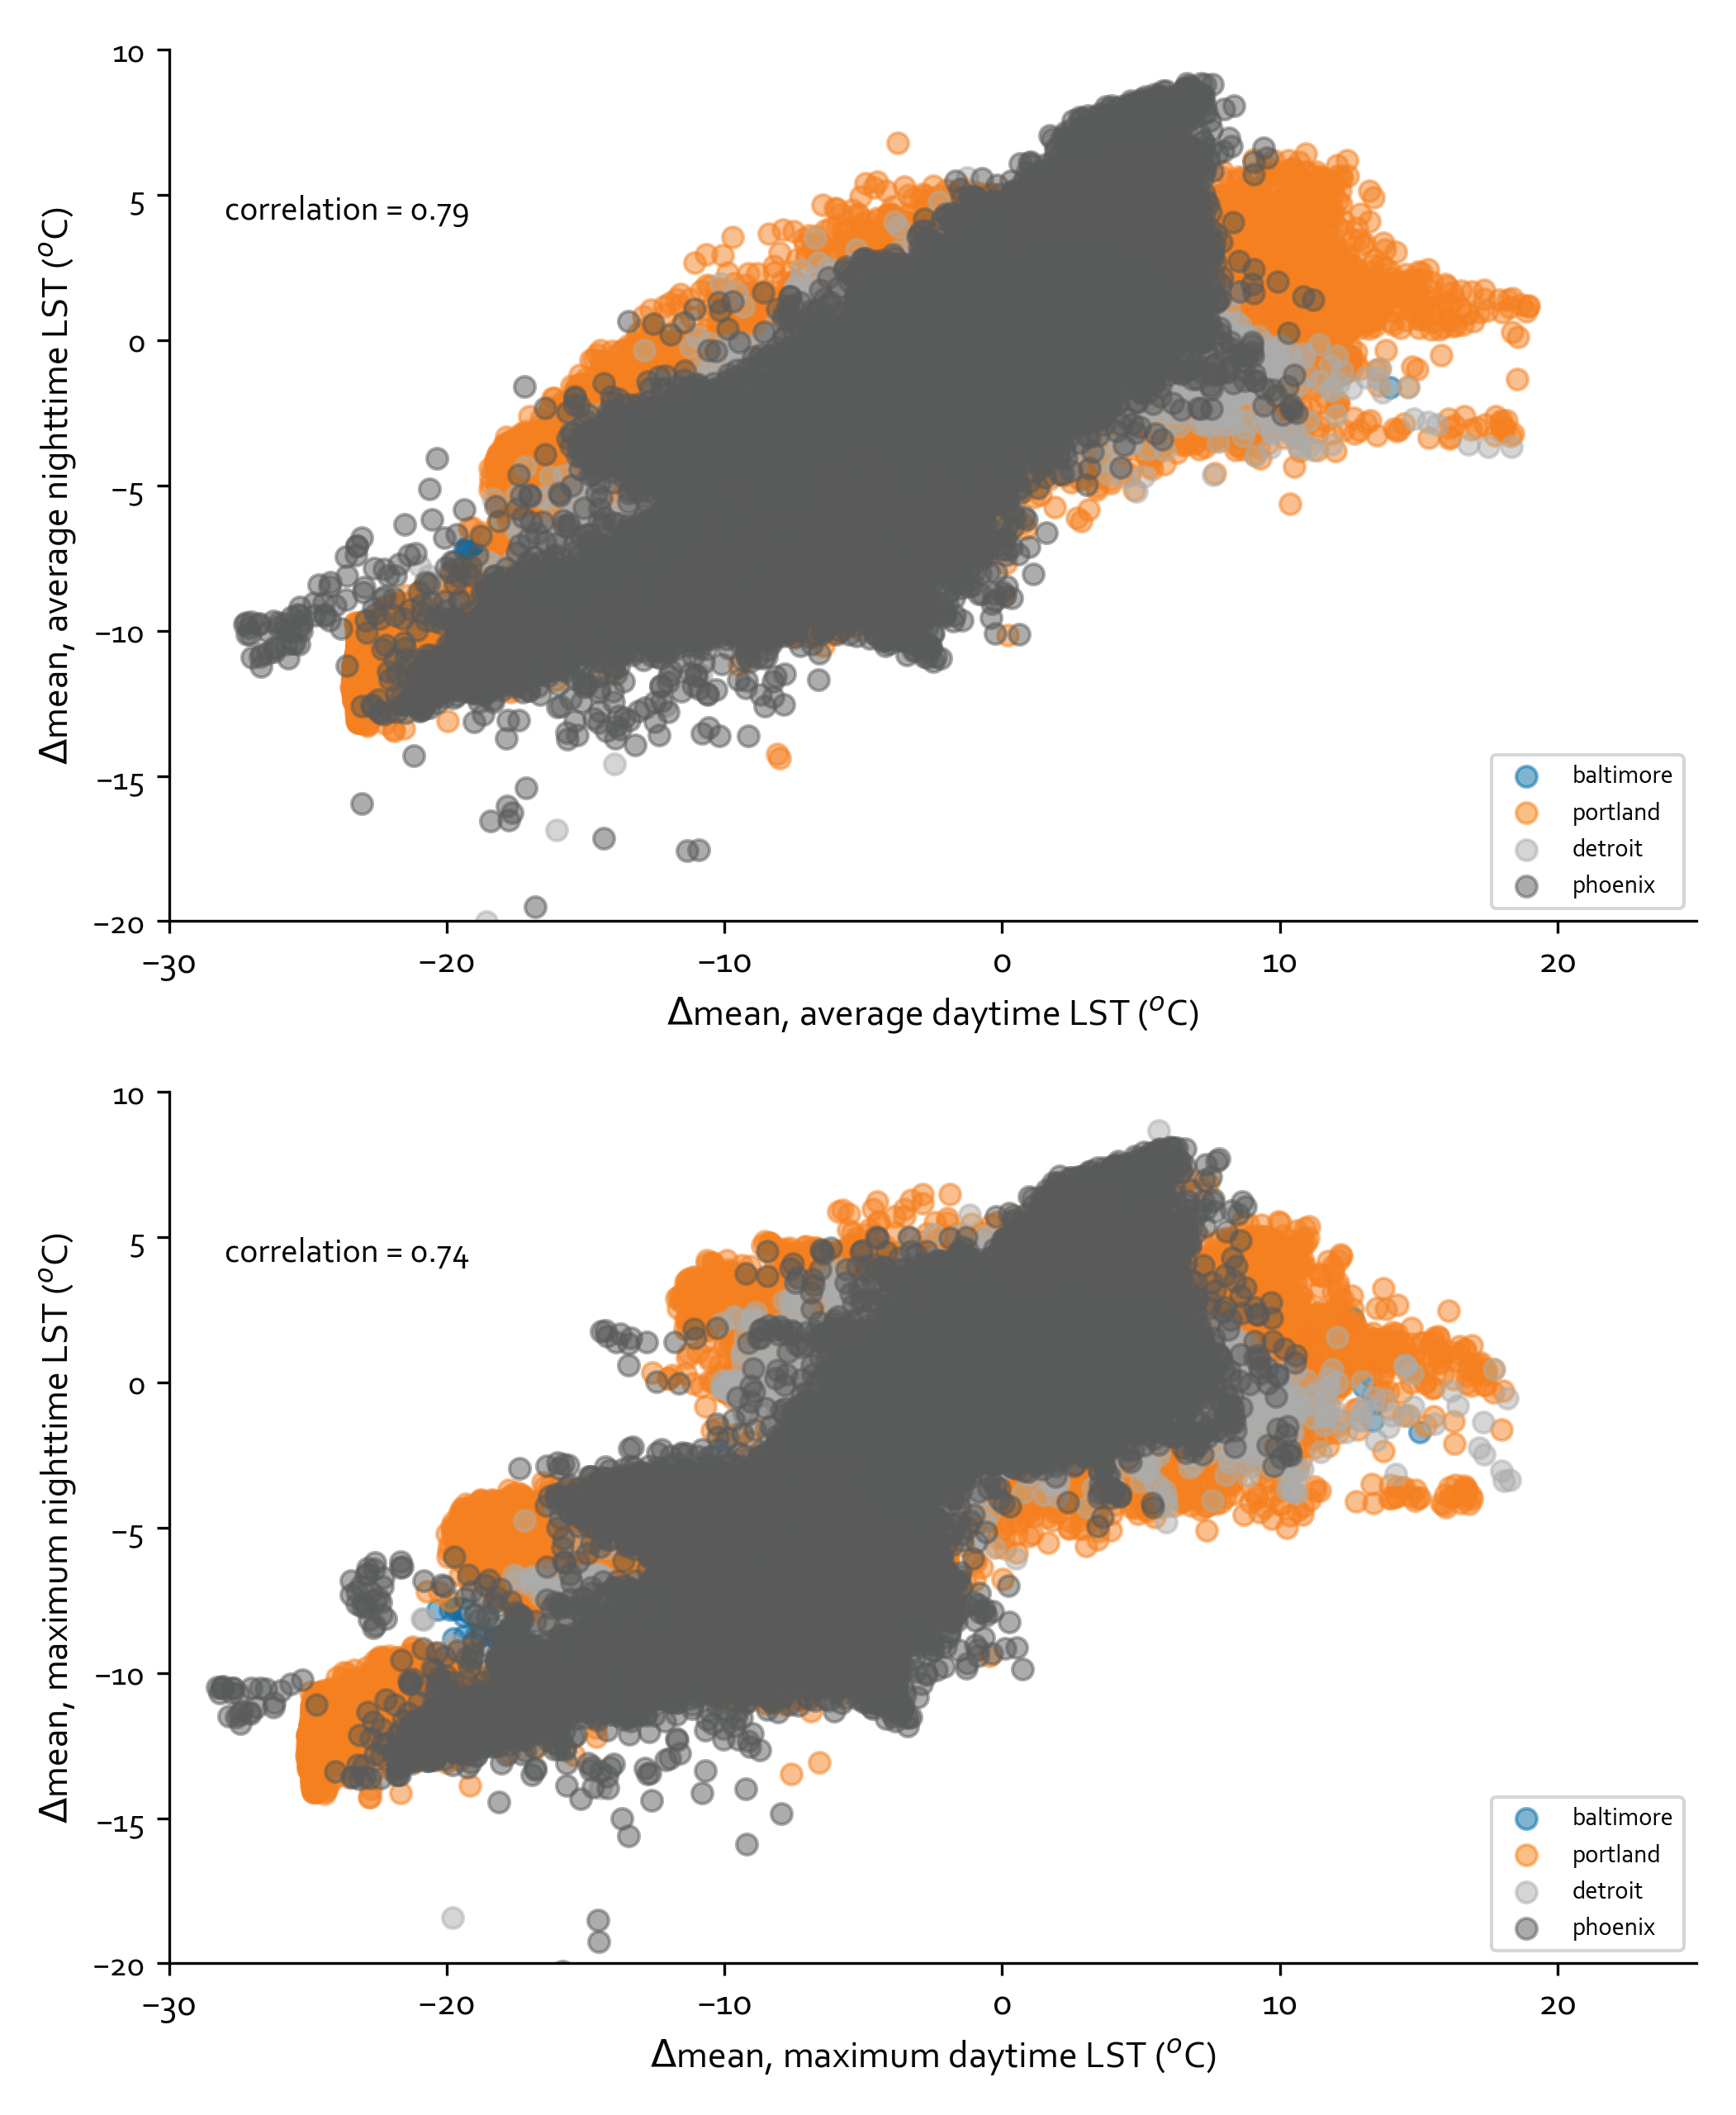
\includegraphics[width=\linewidth]{fig/report/scatter_100.png}
    \caption{The land surface temperature in $^o$C of the cities studied at a 100m square resolution.}
    \label{fig:scatter_lst}
    \end{center}
\end{figure}

\subsection{Independent variables}

\textit{Albedo}. Albedo is a measure of the reflectivity or brightness of a surface. It is normalized between 0-100 where the darker surfaces are lower values. Albedo is calculated using the LandSat8 images using the algorithm described in \cite{Smith2010-nw, Liang2001-jd}. 

\textit{Building floor area}. The building floor area within the cell. This uses data released in 2018 by Microsoft where building footprints are estimated using areal images. 

% \textit{Building height}. Building height is estimated using the building footprints and available lidar data following \cite{Chun2017-mm}. The mean lidar elevation within each building's footprint is subtracted by the mean digital elevation (topography) within the footprint to estimate the building's height.

\textit{Elevation}. 1/3 arc-second (~10m) bare-earth elevation (topography) data is available courtesy the U.S. Geological Survey. 

\textit{Surface elevation}. The surface elevation is determined from the lidar data. Surface elevation captures the natural and built features. 

\textit{Impervious surface percentage}. This is provided in the National Land Cover Database from the Multi-Resolution Land Charasteristic Consortium \cite{Xian2011-aa}. 
To generate the impervious surface area (ISA), the consortium uses LandSat data, NLCD land cover, and nighttime light imagery. 
The stable nighttime light intensity is only used to estimate the boundary of urban areas. 
The Landsat images were converted to top-of-atmosphere reflectance. 
The data is provided at a 30m resolution.

\textit{Land cover}. 
Classification of land cover is described in \cite{Homer2015-ce}. 
However, as it is used in the calculation of emissivity when calculating the LST it cannot be used as an independent variable. 
The only landcover that we use is category 11, water. 

\textit{NDBI}. 
Normalized difference built-up index indicates the intensity of imperviousness \cite{Bhatti2014-ae}. 
It is calculated from satellite images as $$NDBI=\frac{B_{SWIR}-B_{NIR}}{B_{SWIR}+B_{NIR}}$$ where $B_{NIR}$ and $B_{SWIR}$ are the reflectances in the near-infrared and short-wave infrared bands respectively \cite{Alhawiti2016-wv}. 
Using LandSat8 imagery, this is $$NDBI=\frac{B6-B5}{B6+B5}$$ \cite{barsi2014}.
% *Kaplan 2018, Peng 2018

\textit{NDVI}. 
The normalized difference vegetation index (NDVI) measures green vegetation. 
It is calculated from satellite images as $$NDVI=\frac{B_{NIR}-B_{red}}{B_{NIR}+B_{red}}$$ where $B_{NIR}$ and $B_{red}$ are the reflectances in the near-infrared and red bands respectively \cite{Alhawiti2016-wv}. 
Using LandSat8 imagery, this is $$NDVI=\frac{B5-B4}{B5+B4}$$ \cite{barsi2014}.

% \textit{Nighttime light intensity}. Stable nighttime light intensity is available from the Defense Meteorological Satellite Program (DMSP) Operational Linescan System (OLS). They prepare the data to remove clouds and ephemeral light sources. We use 2013 (the most recently available) data of version 4 at a spatial resolution of 30 arc-seconds (1km at the equator) \cite{ngdc2013version}. The nighttime light intensity was found to be only in moderate agreement with density \cite{bagan2018}, meaning lights may indicate anthropogenic energy use during the night. However, it's lower resolution means that can not capture minor differences. We resampled the raster to a 30m resolution, as per the NLDC \cite{Homer2015-ce}, and for each grid calculated the mean, min, and max.

\textit{Population density}. 
Some studies have found that population density has a positive influence on LST \cite{Li2017-yl, Peng2018-cp}, although this may be the result of confounding with other factors. 
We calculate population density using the U.S. census at the block level. 
The most recent census was 2010, so we use that data as an estimator of where people reside in the evening. 
This data is also at a lower resolution that the grid cells used, so the grid cell assumes the density of the block that its centroid is contained within.

\textit{Sky view factor}. Urban canyons have been found to have an effect on UHI because they prevent air circulation and hinder nighttime radiative cooling \cite{Landsberg1981-mq, Chun2017-mm} and are used to indicate radiation flux within complex environments \cite{Matzarakis2007-xy}. We calculate SVF using the R packages \textit{horizon} \cite{Van_doninck2018-ib} that is based off the algorithm presented in \cite{Dozier1990-kn}. 
We use the same parameters used by \cite{Chun2017-mm}: the number of search directions, $\phi=10^o$; and the radius of the reference circle, $R=300m$. 
We use a spatial resolution of 6 meters.
% * Yuan 2011, Unger 2004.

\textit{Tree canopy cover}. 
The 2011 edition of percent tree canopy cover is calculated using National Agriculture Imagery Program (NAIP) aerial imagery, Landsat 5 imagery, elevation, and existing NLCD data \cite{Coulston2012-uu, Homer2015-ce}. 
The data provided is at a 30m resolution. 
The six reflective bands from Landsat 5 are used to calculate top-of-atmosphere reflectance \cite{Coulston2012-uu} so the data does not contain information used in the LST calculation (which requires radiance). 
% * Rogan 2013, Elmes 2017

\subsection{Data preparation and robustness}

The objective of our study is to determine the most influential urban characteristics and understand how they relate to land surface temperature.
To do this, we use partial dependence plots to understand how the urban characteristics are associated with land surface temperature.
For a selected characteristic, partial dependence is calculated by fixing the value of that characteristic in all observations in the dataset and predicting the land surface temperature. 
This is repeated over a range for the feature of interest.
To evaluate how multiple urban characteristics interact, partial dependence can also be conducted in multiple dimensions.
The swing \cite{Shortridge2015-ub} measures the relative importance of variables by calculating the magnitude of change in temperature associated with each variable.
To calculate partial dependence, we need a data set and a statistical model.

To analyze the data, it needs to be transformed into a suitable format that is consistent between the variables.
The raw data is a variety of spatial data types from ``area level" (the population density data), to ``geostatistical raster" (e.g. the land surface temperature).
We choose to resample the data into a grid of square cells.
We conduct the resampling twice to produce a grid of 100 and 500-meter square cells. 

Having two resolutions allowed us to evaluate whether our conclusions are robust.
For each of the cells the mean, maximum, and minimum of all variables were calculated. 
To further account for spatial effects of each variable, the mean of the surrounding cells (including diagonal) was calculated and the resulting spatial lag variable was included as an additional independent variable. 
To address multicollinearity between the variables that would confound our analysis of influence, we remove variables iteratively that have a Variance Inflation Factor greater than 5.
The result is a data set with which we can train statistical models.

Various statistical models (\S \ref{ss:models}) were trained and then validated on unseen data using a technique known as holdout cross-validation. 
This approach partitions 80\% of the data into a training set and the remaining 20\% into the testing set.
The model resulting from the training is then tested on this unseen test set (known as out-of-bag) to get an estimate of the model accuracy.
This is repeated 100 times and the distribution of the accuracy metric (here we use the mean absolute error (MAE) and variance explained (R$^2$)).
Holdout cross-validation of this type is crucial for statistical analysis to ensure that models are not overfit to data \cite{Geron2017-ek}.
Over fitting occurs when a model fits to the randomness in a dataset, causing it to be unsuitable for generalizations. 
When models' accuracy metrics are reported based on in-sample data (the same data it was trained on), the accuracy metrics are high.
Avoiding overfitting is therefore essential when working with statistical models and is overlooked by the majority of existing studies.
Cross-validation helps to avoid this by evaluating the model on unseen data.

A further way to avoid overfitting is to carefully consider how the test data is selected.
This is especially important with spatial data.
Therefore, when selecting the test and training data the grid cells were grouped into a larger 8x8 grid.
This avoids overfitting of the model by training the model on a cell adjacent to a cell that is included in the test set.

Finally, we attempt to capture uncertainty in the data and the models. 
To represent the data uncertainty, we draw a random sample from our data, with replacement, to simulate a new dataset.
The models are trained on this new dataset and this is repeated.
This approach, known as bootstrapping, means that the conclusions' sensitivity to the data can be assessed.
If the results are vastly different for each bootstrap sample, we assume that the result is dependent on the data and is unlikely to be generalizable to other cities.
Additionally, we capture model uncertainty by using different models and assessing how each model shows the urban characteristics influencing the land surface temperature.
If all bootstrapped models are generally in agreement, it suggests that the conclusions are robust.


\subsection{Statistical models}
\label{ss:models}
The relationship between urban characteristics and land surface temperature is complex.
This complexity may not be captured by a linear regression model. 
We fit a series of regression and data-mining models to the data and their predictive accuracy and variable association are compared.

It is important to note that we are assessing the association between the urban characteristics and the land surface temperature.
These models are not explicitly evaluating causality. 
Instead, we use these models to control for urban characteristics and evaluate how land surface temperature changes with changes in each of the other urban characteristic in turn.

\textit{Null model: average}. The first model, to compare other models against, is the null model. 
This is a benchmark model to ensure the models we fit are not doing worse than no model.
The mean of the observations in the training set is calculated and is used as the prediction for the test observations.

\textit{Linear model}. Linear models are suitable when the relationship between the explanatory variables (urban characteristics) and the response variable (LST) is linear. 
That is, linear models take the form $$ y = \beta_0 + \sum_i \beta_i x_i + \varepsilon$$ where $y$ is the response (LST), $x_i$ is each for the variables (urban characteristics), $\beta_0$ is the intersection, $\beta_i$ is how the LST changes linearly with each urban characteristic, and $\varepsilon$ is the normally distributed error.

\textit{Multivariate Adaptive Regression Spline (MARS)}. 
MARS models are a type of non-parametric regression approach that are useful for high dimensional problems \cite{Hastie2009-ky}. 
They extend the linear model by using piecewise functions to fit the data \cite{Friedman1991-of}: $$ y = \sum_i c_i B_i(x)$$
$B_i(x)$ is the basis function that includes multiple linear functions and indicator variables that set these functions to zero for certain ranges of $x$.
That is, multiple linear approximations are summed across the variable range and provide a nonlinear estimate of the LST \cite{Friedman1991-of}. 

\textit{Generalized Additive Model (GAM)}. 
The GAM is also an extension of the linear model but relaxes the assumption that the relationship is linear \cite{Hastie1990-cg}.
Instead, the response variable is estimated as the sum of smoothing functions, splines, that are applied to each covariate or set of covariates: $$ y = \sum_i s_i(x_i)$$ where $s_i(x_i)$ is the smoothing function applied to each covariate \cite{Shortridge2015-ub}.

\textit{Random Forest}. A random forest is an ensemble model of \textit{Regression Trees}. 
A regression tree partitions the data based on thresholds for the covariates \cite{Breiman1984-hw}. 
The tree continues to `grow' by recursively partitioning the data with the objective of maximizing the node impurity, so that the partitions are as similar as possible. 
The result is a tree-like structure that uses thresholds on the covariates to estimate the response.

We use a total of 500 regression trees.
Each regression tree is trained on a randomly selected subset of 1/3 of the covariates. 
The resulting prediction from the random forest is the unweighted mean of the prediction from all of the trees \cite{Breiman2001-rt}.
A subset of the covariates is used to reduce the correlation between the predictions of each tree.
Tree-based models do not assume linearity and so are generally very flexible and powerful models \cite{Breiman2001-rt, Geron2017-ek}.

\textit{Gradient Boosted Regression Trees}. 
GBRT's are also a collective of regression trees. 
In contrast to random forest models, each tree is trained sequentially on the residuals of the previous tree.
That is, each regression tree has the objective of reducing the error of the previous tree.
The prediction from the GBRT is the unweighted mean of all of the regression trees \cite{Geron2017-ek}.
In this case, we again use 500 trees.

\textit{Convolutional Neural Network}. 
CNN's are a new technique in deep learning and have most commonly been used to analyze visual images.
Their use in image processing makes them potentially suitable for geographic studies.
As with other forms of neural networks, CNN's contain layers of mathematical functions (neurons) that operate on the independent variables \cite{Geron2017-ek}.
There can be multiple layers of these neurons that pass the results as an input to subsequent layers.
In this manner, neural networks can capture nonlinearities.
The advantage of convolutional neural networks above other types of neural networks is their ability to capture the spatial dependencies. 
Because CNN's have seldom been used for geospatial data, we provide a more detailed explanation in (\ref{ss:cnn}).

\section{Results and Discussion}

\begin{figure*}
    \centering
    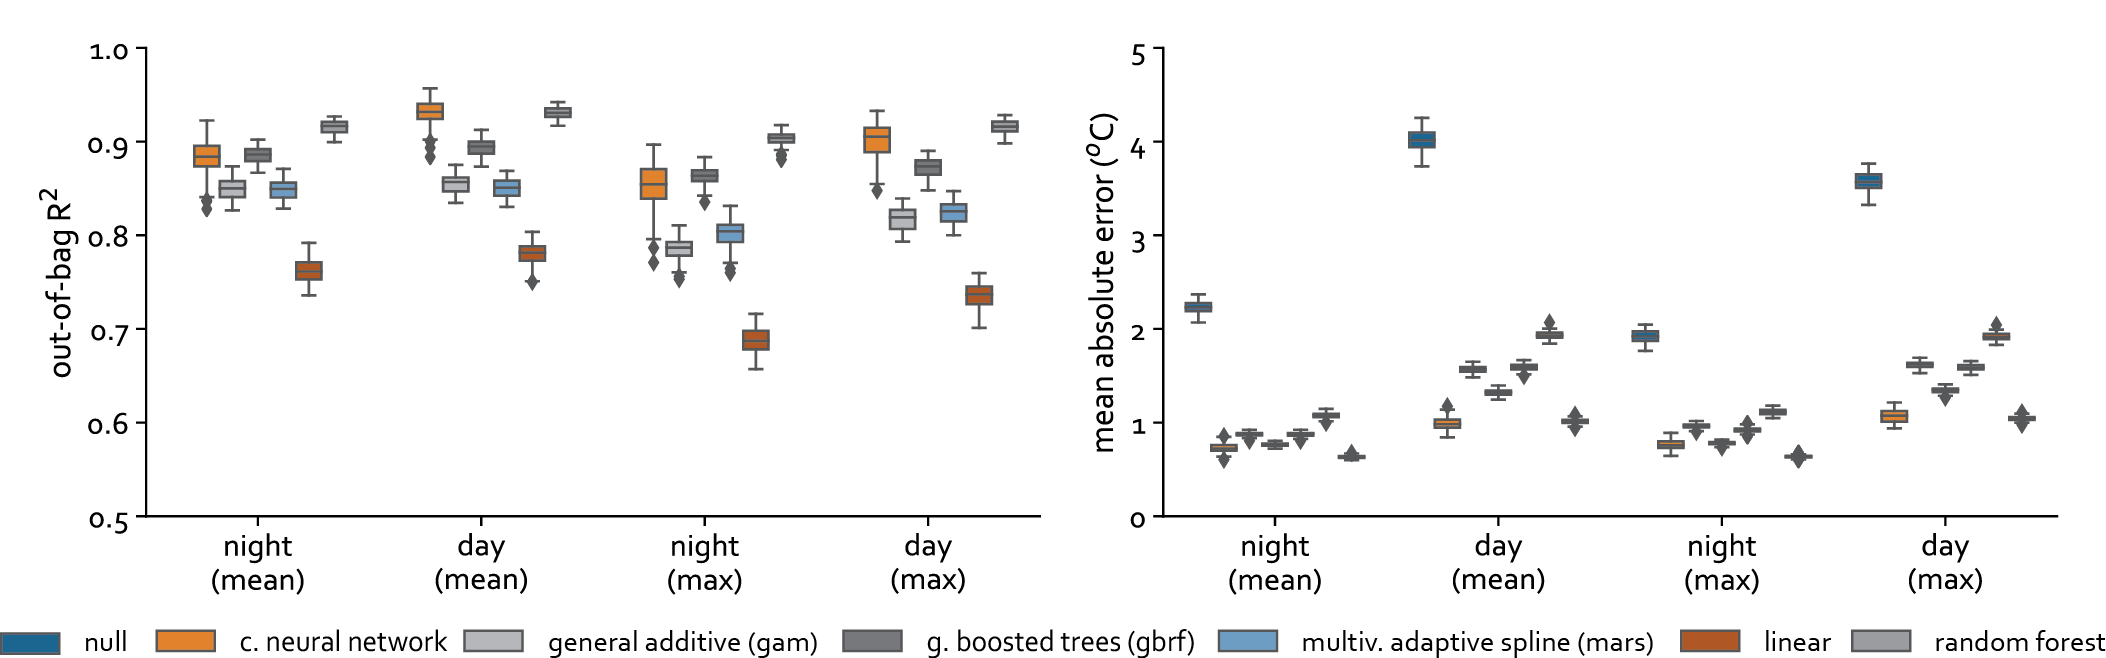
\includegraphics[width=\linewidth]{fig/report/holdout_100.png}
    \caption[Holdout cross-validation results at 100-meter resolution]{
    Holdout cross-validation results at 100-meter resolution.
    The out-of-bag (OOB) R$^2$ and mean absolute error (MAE) of the models from a 100-fold holdout cross-validation. 
    The models were trained on 80\% of the data and tested on the unseen 20\%.
    When selecting data for the training and testing sets, spatial subsets were used to account for spatial similarities. 
    OOB R$^2$ can vary between $(-\infty, 1)$, where better models have a value near 1. 
    Good models have MAE near 0.
    }
    \label{fig:holdout_100}
\end{figure*}

In this study we seek to determine the influence and relative importance of urban characteristics on land surface temperature during both the day and night.
To achieve this, we first select variables to remove based on collinearity. 
The remaining variables for both 100 and 500-meter resolution analysis are shown in \ref{tab:vif}. 
The next phase is to assess the accuracy of the statistical models.
The results in Figure \ref{fig:holdout_100} show that the best models can predict both day and night land surface temperature to within 1$^o$C using urban characteristics.
The R$^2$ results, also based on unseen data, suggest that more than 90\% of the data variance is captured by the best models.
We find that the most accurate model is the random forest, closely followed by the gradient boosted regression trees and convolutional neural network.
The weakest model, consistently with R$^2$ less than 80\%, is the linear regression - incidentally the model that is used in the majority of existing studies into land surface temperature.
These results allow us to assess the influence and relative importance that these characteristics.

\begin{figure*}
    \begin{center}
    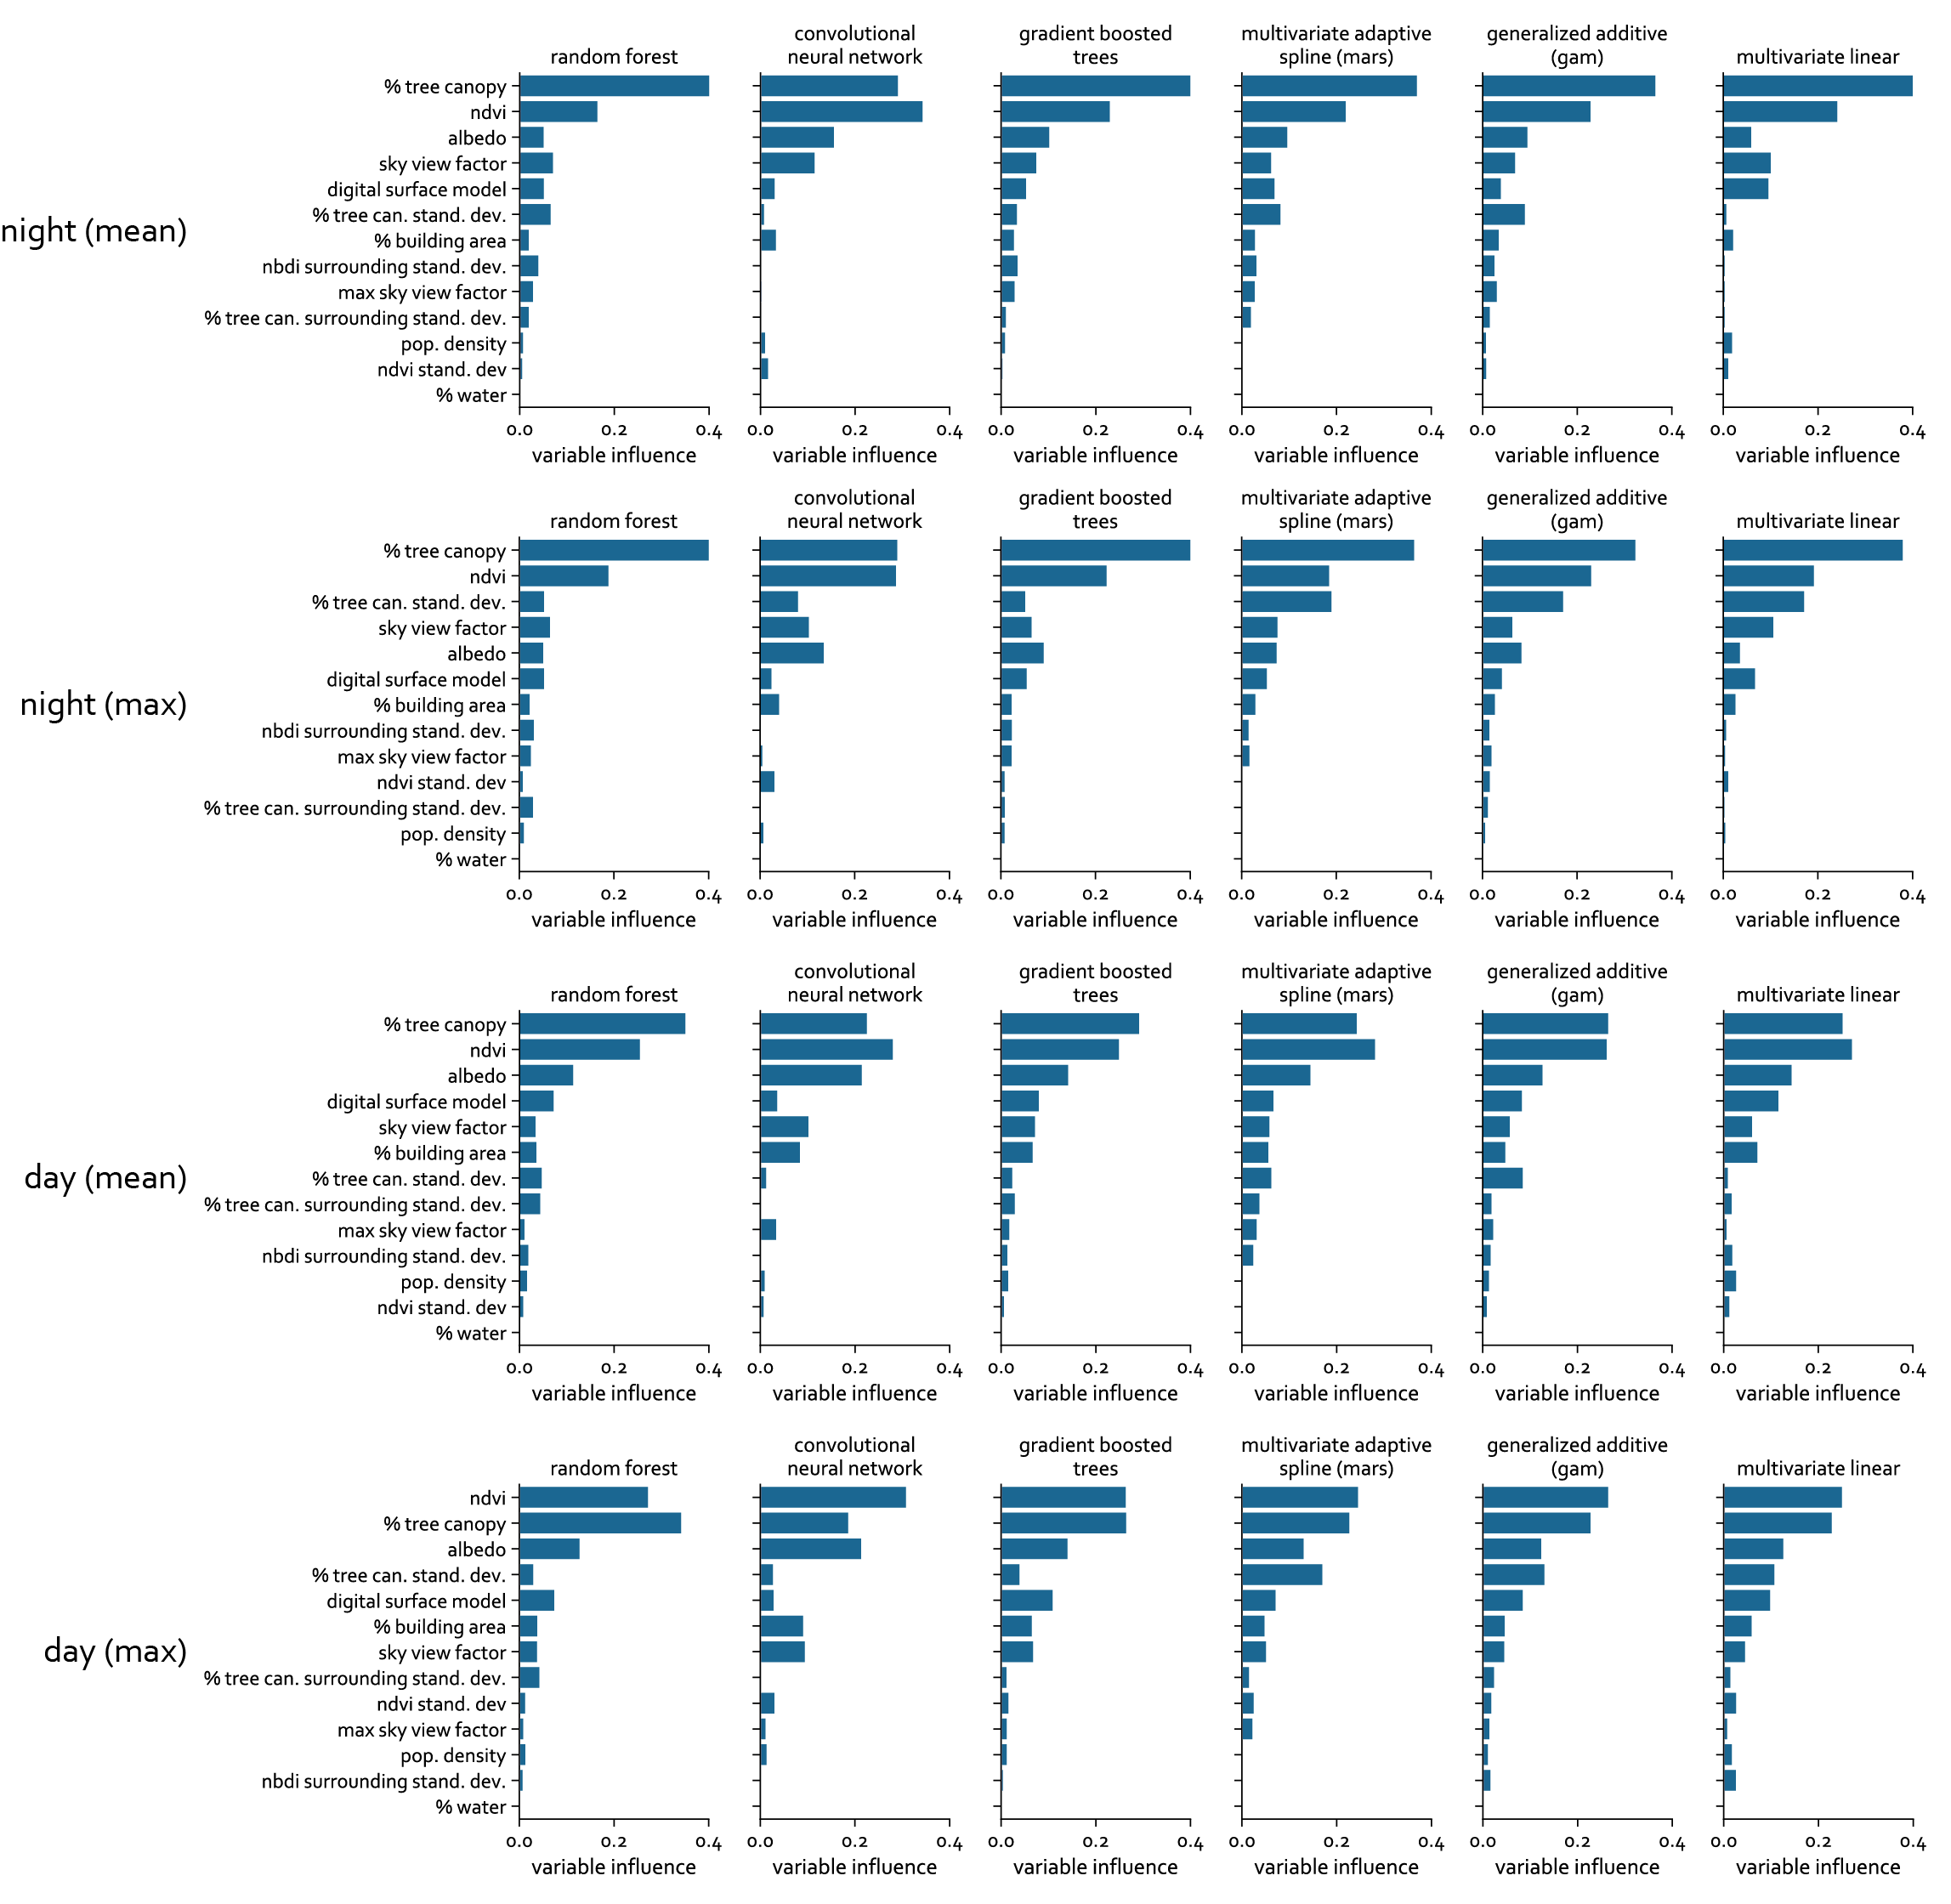
\includegraphics[width=\linewidth]{fig/report/importance_100.png}
    \caption[Variable influence on LST at 100-meter resolution]{
    Variable influence on LST at 100-meter resolution.
    The variable influence, measured by swing, shows the relative importance of each urban characteristic on land surface temperature.}
    \label{fig:importance_100}
    \end{center}
\end{figure*}

\begin{figure*}
    \centering
    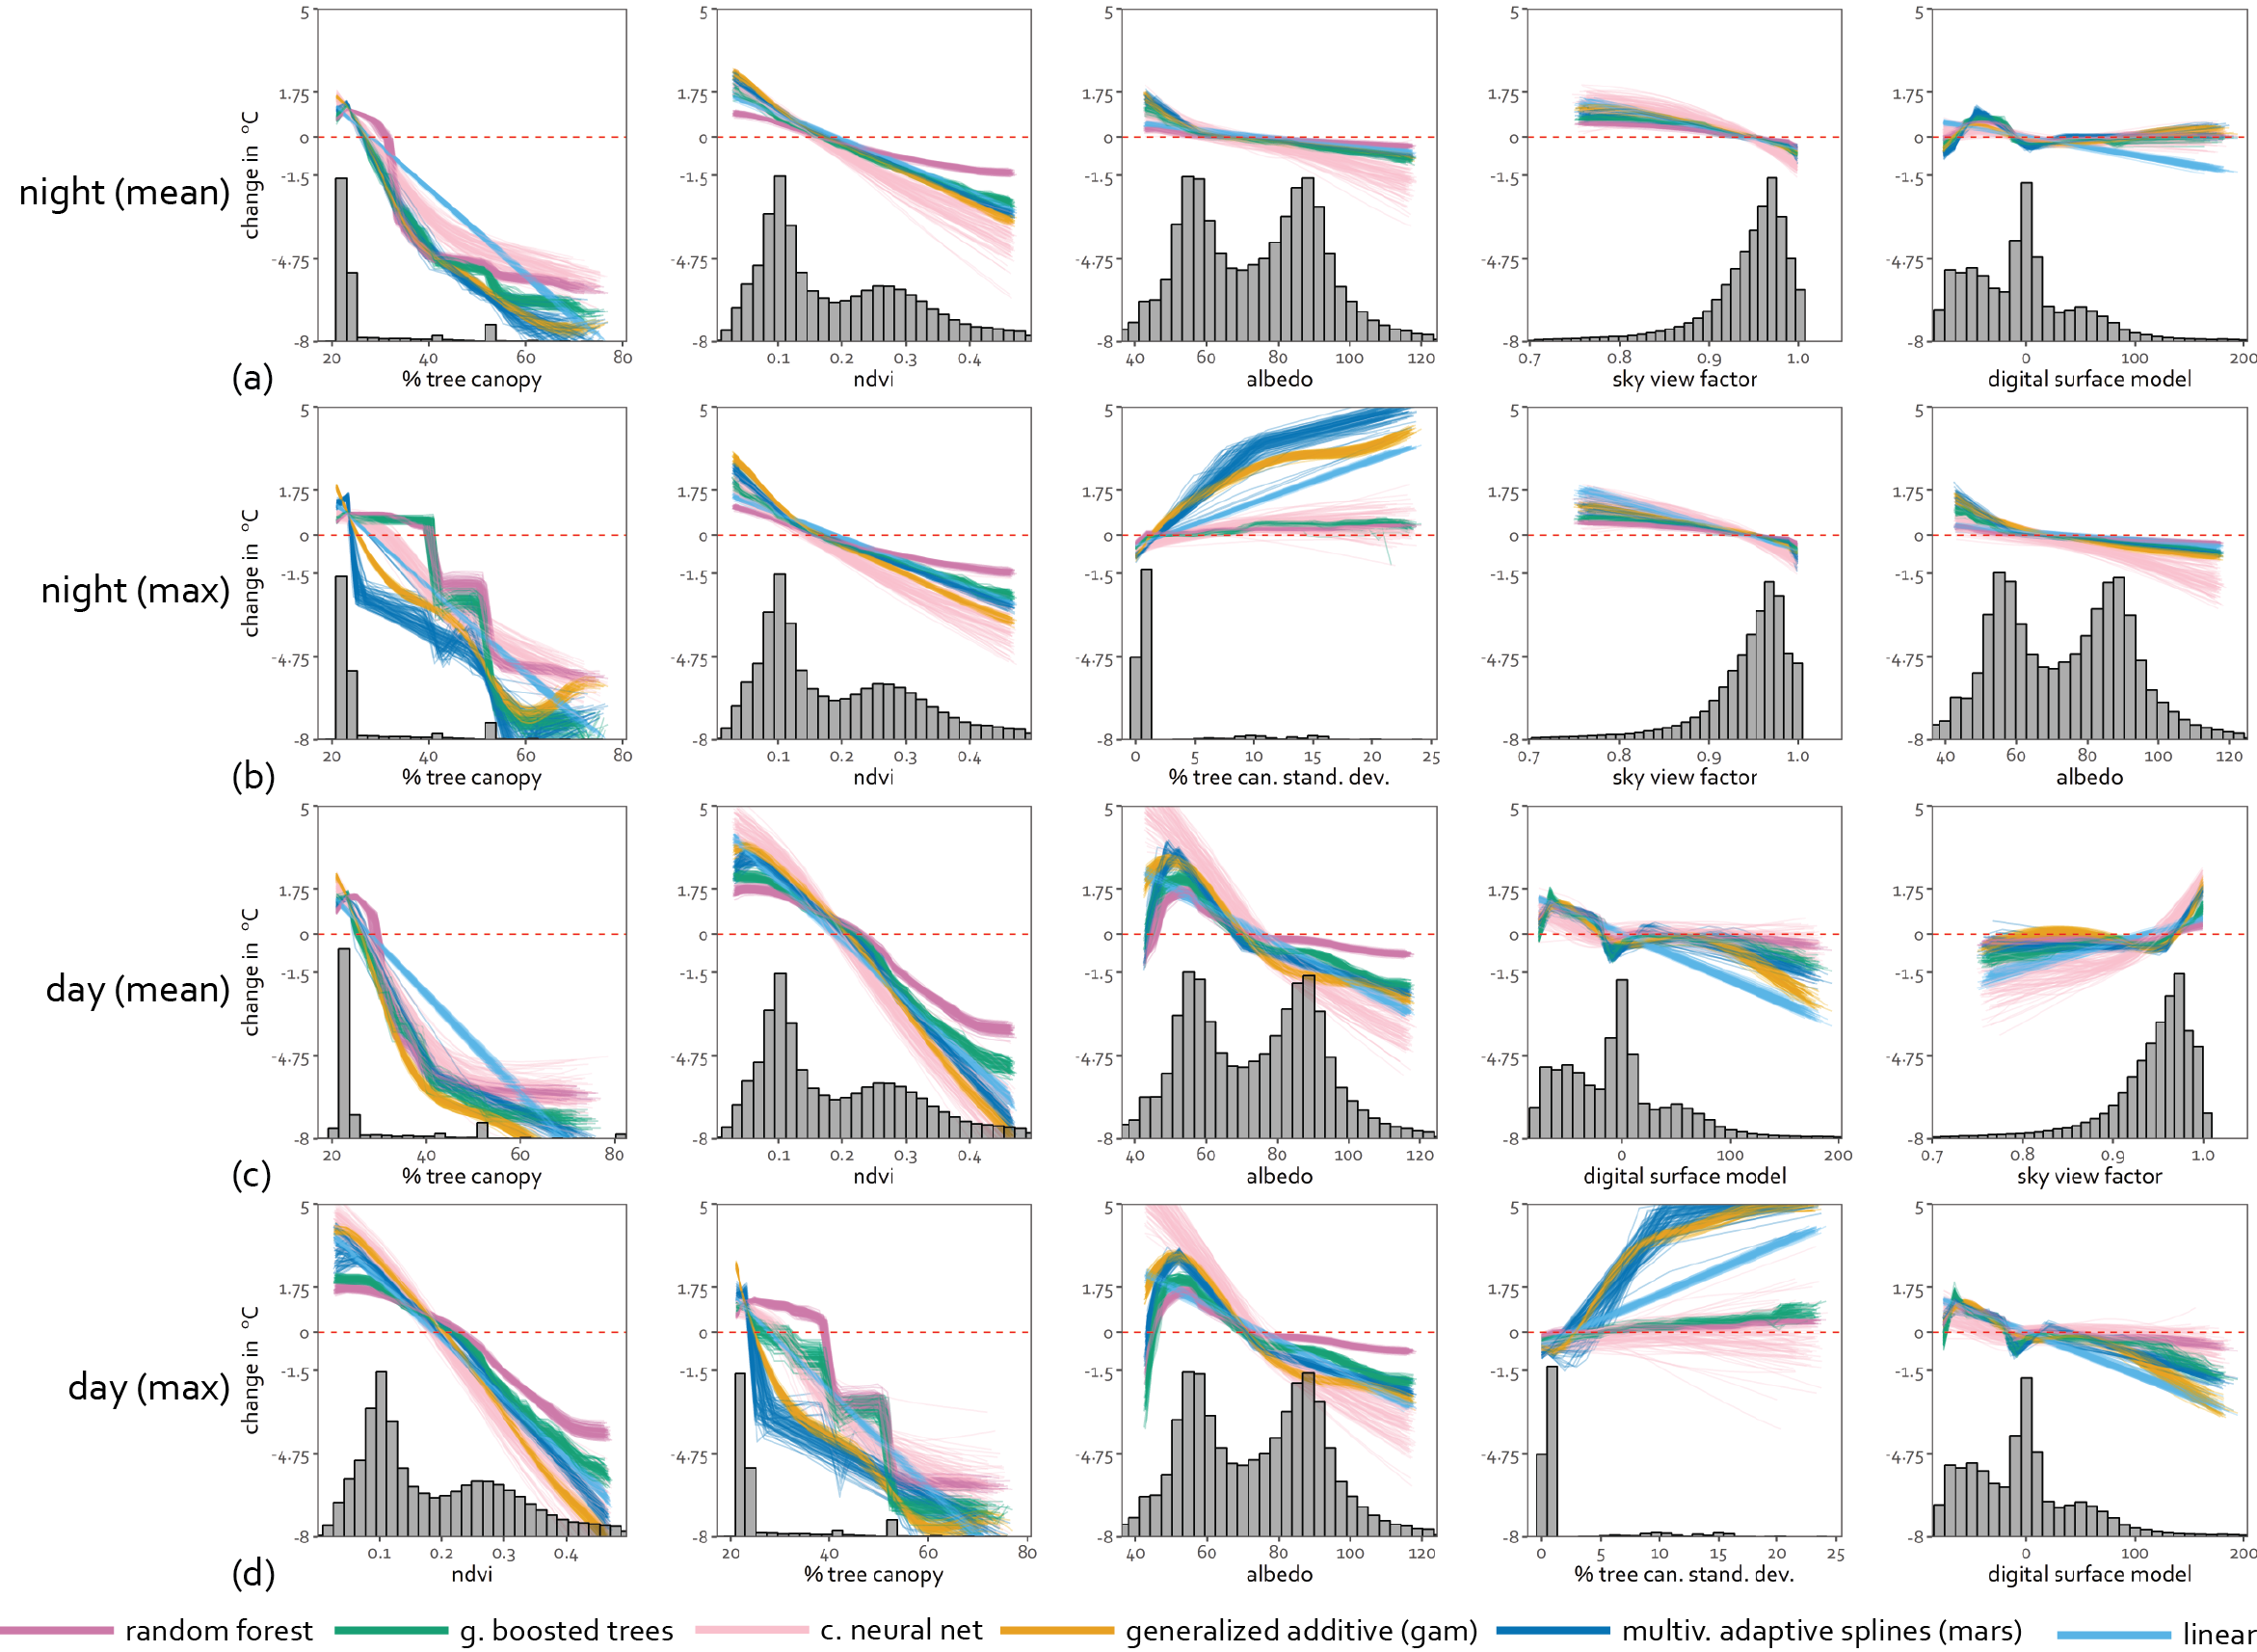
\includegraphics[width=\linewidth]{fig/report/pdp_100.png}
    \caption[Partial dependence plots for LST at 100-meter resolution]{
    Partial dependence plots for LST at 100-meter resolution.
    Partial dependence plots show how the land surface temperature ($^oC$, y axis) changes with each urban characteristic as the other variables are held at their average (mean) value. 
    The left hand side shows the effect each variable has on the (a) mean land surface temperature (LST) during the night, (b) maximum LST during the night, (c) mean LST during the day, (d) maximum LST during the day. 
    Each of the models are shown and this indicates the model uncertainty in the relationships.
    There are multiple lines for each model based on bootstrap samples of the data, which indicates the data uncertainty.
    The histograms on the $x$-axis shown the distribution of the observed data.
    This is for the 500-meter resolution.
    }
    \label{fig:pdp_100}
\end{figure*}


Relative variable importance for all the urban characteristics, calculated with \textit{swing}, is shown in Figure \ref{fig:importance_100}. 
The characteristics, shown on the $y$ axis, are ordered by the mean swing across all of the models, and the models are ordered left-to-right by their cross-validated accuracy.
The most important characteristics during the night are tree canopy cover, greenness (NDVI), the sky view factor, and the elevation (digital surface model).
The albedo is found to be important when assessing the 100-meter data, while the \% area covered in water is important with the 500-meter data.
This is likely due to 98\% of the cells at 100m resolution having 0\% water, so the effect on the dataset is negligible.
The important urban characteristics are consistent for both the mean and maximum temperature during the night.
The characteristics are also relatively consistent between night and day and between the models. 
Although albedo is among the top factors, its relative importance is low compared to tree canopy and greenness, especially during the night. 
This low association with nighttime temperatures is surprising given that darker surfaces store heat during the day that is released during the night \cite{Voogt2003-mm, Zhou2014-wc}.
This, and the other influences can be examined using partial dependence.

\textit{Vegetation and impervious surfaces}. 
During the day, increasing impervious surfaces and decreasing vegetation causes increased sensible heat flux and lowered latent heat flux \cite{Voogt2003-mm, Peng2012-iy, Zhou2014-wc}.
This is thought to be less important during the night because latent and sensible heat are dominant during the day, but ground heat flux dominates at night \cite{Zhou2014-wc, Voogt2003-mm}.
Indeed, because transpiration does not occur at night, vegetation's effect on night temperatures is debated. 
In our study, percentage tree canopy and impervious surface cover must be discussed together because they are 100\% correlated in the data (Figure \ref{fig:imp_tree}).
To distinguish between vegetated surfaces and other pervious surfaces, we include NDVI, a measure of a surface's greenness.
At night, we find that \% tree canopy (and \% impervious surface) is the most influential characteristic on land surface temperature, followed by NDVI (Figure \ref{fig:importance_100}).
The partial dependence results (Figure \ref{fig:pdp_100}) indicate a decrease in up to 10$^oC$ as the percentage area of trees or other pervious surface increases.
This reduction in temperature could be due to a reduction in the impervious surfaces that store heat.
We also observe that as the NDVI increases, the land surface temperature decreases.

To further evaluate whether the influence with temperature is due to vegetation or pervious surfaces, consider the the two-dimension partial dependence (Figure \ref{fig:pdp_2dnight_100}d) that evaluates how LST varies with \% tree canopy/impervious surface and the NDVI.
The greener (higher NDVI) and more pervious (higher \% tree canopy cover) a surface is, the cooler it is during the night. 
The total change here is also approximately 7.5$^oC$, which is a considerable amount given these two-dimensional partial dependence are calculated using the random forest model, which is the less sensitive of the five models (as seen in Figure \ref{fig:pdp_100}).
These results contradict standing conclusions that vegetation has no effect on nighttime LST \cite{Peng2012-iy, Zhou2014-wc};
although much of the reduction in temperature could be due to the perviousness of the surface, lowered temperatures appear to be associated with the greenness (NDVI) of a surface during the night.

During the day, we again see that vegetation and impervious surfaces are associated with the greatest reduction in land surface temperature, with approximately 15$^oC$ change (Figure \ref{fig:pdp_2dday_100}: ndvi vs. \% tree canopy). 
This daytime result is consistent with expectation \cite{Chun2017-mm, Peng2018-cp, Wang2019-tree,Zhou2014-wc, Chun2018-so}.
Because not all pervious surface types have the same cooling potential, and because of trade-offs with irrigation of vegetated surfaces \cite{Gober2009-im}, understanding the ideal vegetated surface type for day and night temperatures is a future step.

\textit{Water}.
Water is widely expected to decrease the LST during the day \cite{Wicki2017-fv, Zhou2018-iy, Wang2019-water}, but some claim it increases LST during the night \cite{Chun2017-mm}.
The rationale is that water releases heat during the night, resulting in elevated nighttime temperature \cite{Chun2017-mm}.
Our findings, however, show that water reduces the LST during both the day and night (Figure \ref{fig:pdp_500}).
Although these results are not supported at the 100-meter resolution because 98\% of the data at the 100-meter level has zero percentage water.
At the 500-meter resolution, we see that the presence of water can decrease LST between 1.5 and 8$^oC$ during the night and by substantially more during the day (Figure \ref{fig:pdp_500}).

\textit{Urbanization}.
Urbanization can lead to heat storage in roads and buildings \cite{Zhou2014-wc, Voogt2003-mm}. 
We discussed the role of impervious surfaces, alongside the effect of vegetation, but we also considered the influence of albedo (the whiteness of a surface), the percentage area of building, the NDBI (built-up index), and the sky view factor (a measure of the urban canyon effect).
The results for albedo are surprisingly low.
During both the night and day, albedo has a negative effect on temperature.
During the day, this is most pronounced, and whiter surfaces appear to be more than 5$^o$C cooler than darker ones (Figure \ref{fig:pdp_100}).
The partial dependence plot (Figure \ref{fig:pdp_100}) also indicates that albedo's influence on temperature is potentially confounded as both vegetation and impervious surfaces can be dark surfaces (with low albedo).
This stresses the importance of statistical techniques for evaluating the effect of multiple variables.
We can investigate this further using the 2D partial dependence; the highest temperature occurs when there are dark impervious surfaces, but dark vegetated surfaces are cool (Figure \ref{fig:pdp_2dnight_100}).
Additionally, we see that albedo has little affect at night, although the highest temperature does occur when there is high acreage of building footprint with low albedo (Figure \ref{fig:pdp_2dnight_100}a).
During the day, albedo has a greater influence: increasing the whiteness decreases the temperature (Figure \ref{fig:pdp_100}).
The highest temperatures are observed when there is significant building area and low albedo (Figure \ref{fig:pdp_2dday_100}a), as well as high impervious area and low albedo (Figure \ref{fig:pdp_2dday_100}b).
This supports existing findings that albedo decreases LST during the day, however, that we find no strong effect during the night contrasts existing reports \cite{Peng2012-iy, Zhou2014-wc}.

The built-up index (NDBI), \% building area, and digital surface elevation model also had relatively minor associations with LST.
The elevation (non-built-up) variable was excluded because it was found to be collinear with other variables; the digital surface elevation model was included and represents the elevation including buildings and vegetation.
However, this elevation only appears to have minor associations with land surface temperature (Figure \ref{fig:pdp_100} \& \ref{fig:pdp_500}).
The building area had no effect during the night and minorly increased temperature during the day (Figure \ref{fig:importance_100}).
Maximum NDBI appears to have a slight positive associated with maximum daytime LST (Figure \ref{fig:pdp_500}), but this effect is not observed at the 100m resolution.
This minor-to-negligible relationship is surprising given that NDBI has been reported as among the most important urban characteristics during the day \cite{Peng2018-cp}.
However, the discrepancy may be due to \% impervious surface area being incorporated already with the \% tree canopy data.

The canyon effect is also often attributed with causing warmer temperatures \cite{Chun2017-mm,Oke1988-re}.
While there was high uncertainty in the models, it appears that during the night, the temperatures decrease as the sky view factor increased (Figure \ref{fig:pdp_100}a,b).
This is potentially due to heat being stored within the canyons (areas with low sky view factors).
This is supported in the two-dimensional partial dependence plot (Figure \ref{fig:pdp_2dnight_100}) where the higher temperatures are observed when there is high \% building area and low sky view factor.
It follows that heat is being captured in the canyons. 
However, compared to the other urban characteristics this has a lesser affect, changing the temperature by approximately 1.5$^o$C.
The effect of the sky view factor during the day is low-to-indiscernible (Figures \ref{fig:importance_100} and \ref{fig:pdp_2dday_100}), but suggests that there are higher temperatures when the sky view factor is high.

\textit{Population density}.
We found that population density had no discernible effect during night or day (Figure \ref{fig:importance_100}).

\textit{Result sensitivity}.
To assess the robustness of the results, we conduct the analysis again at the 500-meter resolution (\ref{ss:500_meter}).
The results are consistent.
Additionally, to ensure that the effects are consistent between cities, we construct the partial dependence plots for each city (\ref{ss:city}).
The partial dependence is similar to Figure \ref{fig:pdp_100}.
Therefore, the consistency between 100 and 500-meter lends confidence to these conclusions.

\textit{Urban strategies}.



\begin{figure*}
    \centering
    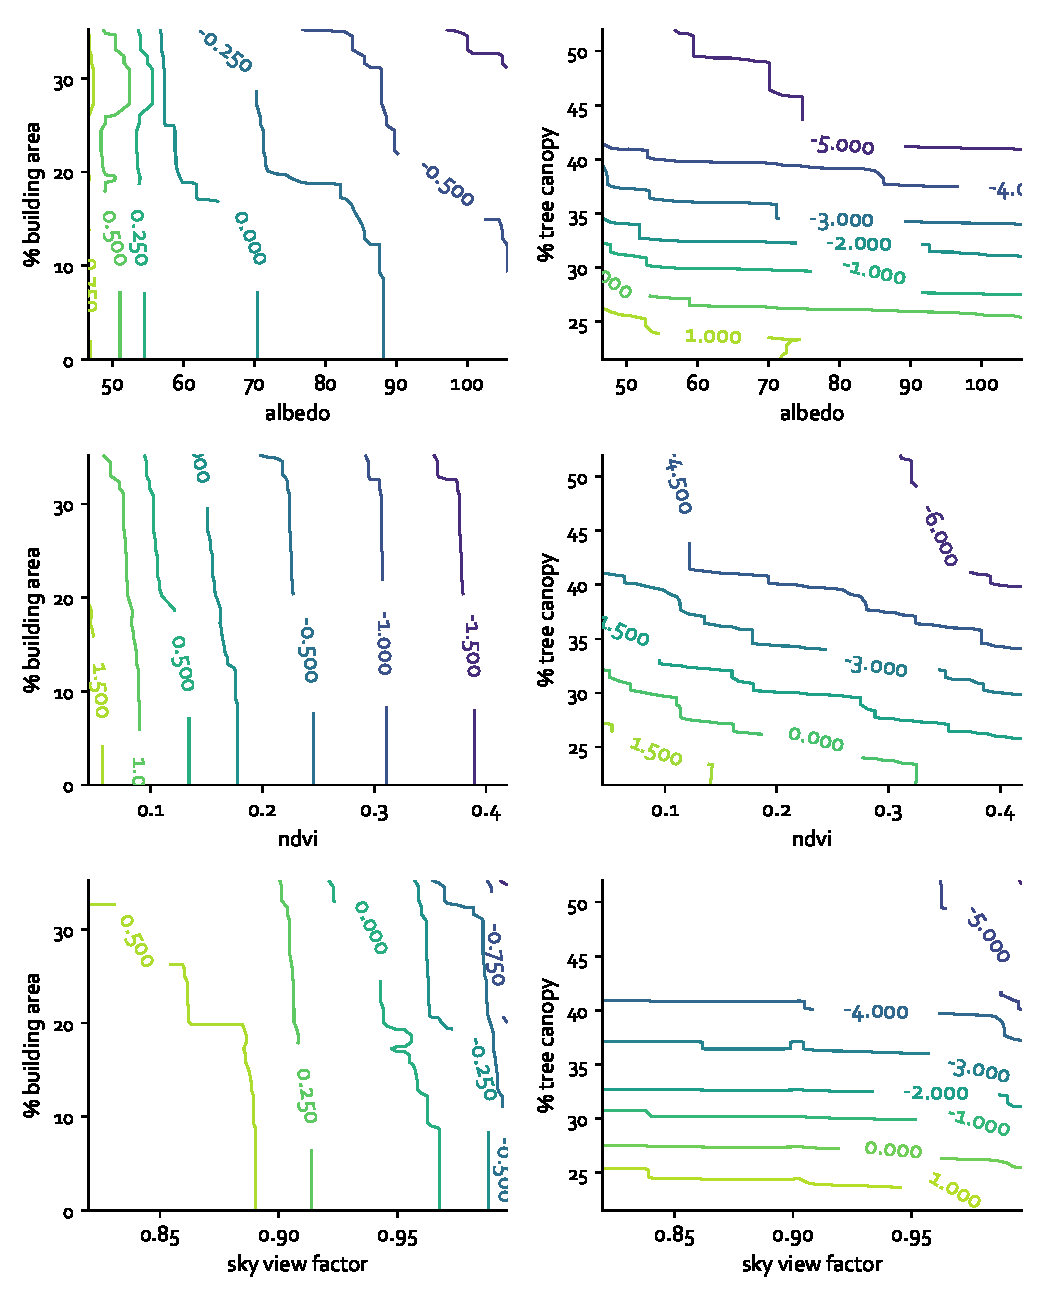
\includegraphics[width=\linewidth]{fig/report/pdp_2d_night_100.pdf}
    \caption{
    \textbf{Nighttime, mean}: A two-dimension partial dependence plot showing how the land surface temperature ($^oC$, contours) changes the variables on the $x$ and $y$ axes, while the remaining variables are unchanged.
    }
    \label{fig:pdp_2dnight_100}
\end{figure*}


\begin{figure*}
    \centering
    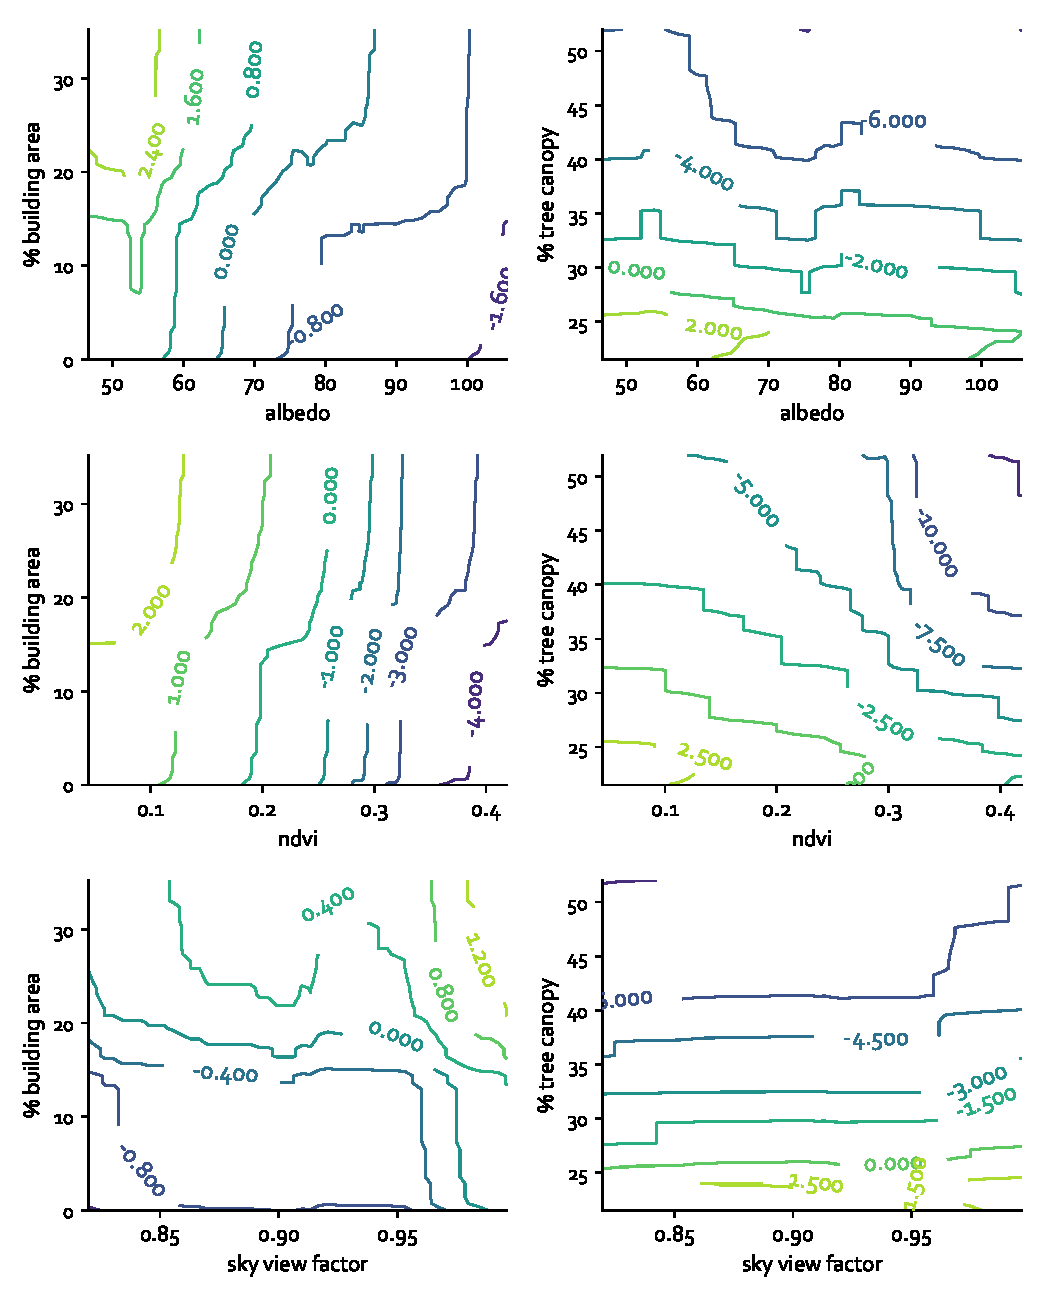
\includegraphics[width=\linewidth]{fig/report/pdp_2d_day_100.pdf}
    \caption{
    \textbf{Daytime, mean}: A two-dimension partial dependence plot showing how the land surface temperature ($^oC$, contours) changes the variables on the $x$ and $y$ axes, while the remaining variables are unchanged.
    }
    \label{fig:pdp_2dday_100}
\end{figure*}


\section{Conclusion}
To assist planners tackling climate change, heat waves, and general high urban temperatures, we seek to determine how different urban characteristics are associated with land surface temperatures. 
The results strongly support initiatives for increasing green infrastructure in cities \cite{Larsen2015-da, Meerow2017-xv}. 
We found that increasing vegetation and reducing impervious surface area had the greatest effect on temperature during both night and day, with the potential to reduce the temperature up to 10$^o$C.
We also see strong evidence for blue space and increasing the area of water, although there are various limitations with doing so in cities such as Phoenix.
We do note that this analysis is for land surface temperature, and not air temperature. 
The correlation between LST and air temperature is not perfect at intra-urban scales, and the magnitude of LST variability tends to be larger  than that of air temperature.
Nevertheless, LST is a highly relevant variable for analyses of the urban energy balance, and thus for studies of the UHI process.

Our findings demonstrate that accurate prediction of land surface temperature using urban characteristics is possible.
This result opens opportunities for further detailed analysis into potential interventions.
Such interventions for mitigating high temperatures are naturally place-specific, and while these results have proven general to four different US cities, work is needed to understand questions such as which types of greenery are better than others \cite{Gober2009-im}.
This study also demonstrates the opportunities of modern statistical techniques and the ability to assess potentially nonlinear interactions and the interactions between multiple variables. 

Rigorous statistical analysis can continue to answer on-going questions central to land surface temperature.
For example, our results support the suggestion that 3D variables (e.g. sky view factor) do not outperform 2D ones (e.g. \% tree canopy cover) \cite{Berger2017-lx}. 
However, iteratively removing these variables from the analysis can ameliorate the potential for conflating the importance of different characteristics \cite{Chun2017-mm}.
Our analysis is not causal inference; such an analysis would require controlled variables and urban spaces.
We instead aim to complement and inform existing understanding of the relationships by demonstrating how land surface temperature and the urban characteristics are associated.
This can be used to inform potential strategies for urban heat reduction, that is, if an association exists between two variables then we can evaluate the potential for causality based on understanding the physical mechanisms.

However, if no association exists or is in the opposite direction of proposed strategies for heat reduction, then such strategies need to be re-evaluated.
For example, our results assessing the relative effect of sky view factor (a measure of building density), population, built-up index, and \% building area do not support claims advocating to constrain floor area ratios \cite{Chun2017-mm}.
Such policy could lead to increased sprawl.
Instead, our results show that reducing impervious area and increasing vegetation and greenness have a stronger association with lowered temperatures.
Such action could be achieved without constraining floor area ratios.
If a constraint is explored, an additional necessary study is to compare sprawling and dense cities, prior to taking steps to dissuade density. 
Now that 100-meter resolution nighttime data is available, as well as the increasing availability of lidar data, studies advocating creative interventions such as increasing the vertical and horizontal randomness of buildings, increasing the prevalence of green roofs \cite{Gago2013-ta}, or other urban planning strategies can quantitatively be explored.

This study into daytime and nighttime land surface temperature in four US cities has highlighted the importance of vegetation in our cities' mitigation options. 
It has also demonstrated the utility of leveraging advanced statistical analysis to study land surface temperature.
The results are robust to both data and model uncertainty and are general across the cities studied.
They suggest that vegetation and impervious surfaces are the most important urban characteristics associated with land surface temperature.
Increasing and decreasing these, respectively, is necessary for reducing high urban temperatures during both night and day.

% There are various bibliography styles available. You can select the style of your choice in the preamble of this document. These styles are Elsevier styles based on standard styles like Harvard and Vancouver. Please use Bib\TeX\ to generate your bibliography and include DOIs whenever available.

% Here are two sample references: \cite{Feynman1963118,Dirac1953888}.
\section*{Acknowledgements}
% TML conducted this research as a graduate student at the University of Michigan with the support of a Rackham PreDoctoral Fellowship.
% The work was also supported by the US National Science Foundation's Grant SEES-1631409. 
% This support is gratefully acknowledged.

\section*{References}
\singlespacing

\bibliography{mybibfile.bib}

\newpage
\onecolumn
\appendix

\section{Data sources}
The data sources for the analysis are listed in Table \ref{tab:data}.

\begin{table}[H]
\caption{The data sources for the LST analysis.}
\label{tab:data}
\fontsize{8}{11}\selectfont
\begin{tabu}to \textwidth{ X[l]  X[c]  X[c] X[l] X[l] }
\toprule
 Data Provider & Data Type & Data Date & Description & Source \\
 \hline
U.S. Geological Survey  & Raster  & 2013-2017 &
    Landsat 8 day and night satellite imagery & \url{https://earthexplorer.usgs.gov/} \\
Microsoft  & Polygon  & 2018 & Building footprint polygons for the US &
    \url{https://github.com/Microsoft/USBuildingFootprints} \\
Defense Meteorological Satellite Program  & Raster  & 2013 &
    Stable nighttime light intensity & \url{https://www.ngdc.noaa.gov/eog/dmsp/downloadV4composites.html} \\
Multi-Resolution Land Characteristics Consortium  & Raster  & 2011 &
    Land cover & \url{https://www.mrlc.gov} \\
Multi-Resolution Land Characteristics Consortium  & Raster  & 2011 &
    Percent developed imperviousness & \url{https://viewer.nationalmap.gov} \\
Multi-Resolution Land Characteristics Consortium  & Raster  & 2011 &
    Percent tree canopy cover & \url{https://viewer.nationalmap.gov} \\
U.S. Geological Survey  & Raster  & 2015 & 1/3 arc-second elevation &
    \url{https://nationalmap.gov/3DEP/3dep_prodserv.html} \\
U.S. National Oceanic and Atmospheric Administration  & Lidar  & 2014 & Point cloud of surface elevation &
    \url{https://coast.noaa.gov/htdata/lidar2_z/geoid12b/data/6377/} \\
IPUMS NHGIS  & Area Level  & 2010 &
    Block-level population from the US census & \cite{nhgis}\\
\bottomrule
\end{tabu}

\end{table}


\newpage
\section{Covariates included in models}

We select variables to include in the model based on the variance inflation factor (VIF). 
This approach removes variables that exhibit high multicollinearity, that is the variable can be predicted from a combination of other variables. 
It is important to remove variables with high multicollinearity in inferential studies because otherwise the variables may confound the effect of one another on the variables of interest.



\begin{table}[h]
% \small
% \fontsize{8}{11}\selectfont
\centering
\caption{Covariates included after accounting for multicollinearity.}
\label{tab:vif}
\begin{tabular}{p{0.23\linewidth} p{0.7\linewidth}}
\toprule
       \textbf{Resolution} & \textbf{Included variable} \\
\midrule
100-meter  & Albedo mean \\
& NDVI mean \\
& Sky view factor mean \\
& \% tree canopy stand. dev. spatial lag \\
& \% tree canopy stand. dev. \\
& NDBI stand. dev. spatial lag \\
& \% building area\\
& Sky view factor max \\
& \% tree canopy mean \\
& NDVI stand. dev. \\
& \% water area\\
& Digital surface model mean \\
& Population density mean\\
\hline
500-meter & NDVI mean \\ 
& Albedo mean \\
& Sky view factor mean \\
& Digital surface model stand. dev. \\
& \% building area\\
& \% tree canopy mean \\
& \% water area\\
& Sky view factor max \\
& NDBI max \\
& \% tree canopy max \\
& Population density mean\\
& Digital surface model mean \\
& \% tree canopy min \\
\bottomrule
\end{tabular}
\end{table}


\newpage
\section{Technical appendix: convolutional neural network}
\label{ss:cnn}
\subsection{Overview}

Our CNN model was adapted from a U-Net architecture \cite{unet}. This architecture is commonly used for image segmentation: the input to a U-Net model is a 2D greyscale image, and the output is another 2D image with values representing the classification of each pixel. The novel property of a U-Net CNN is that the internal layers learn at various resampled resolutions of the input data, which makes the model good at learning phenomena that are driven at multiple scales.

Several modifications were made to adapt U-Net to a geospatial use-case, and are outlined below.


\subsection{Data preparation}

The gridded data for each city was treated as an image, with each pixel representing a 100m or 500m cell. Instead of having three channels (red, green, and blue) like a colour image, these images had one channel for each of the independent variables in the dataset. The target was a 2D single channel image of the same shape.

CNNs require all inputs to be the same shape, which isn't the case for our city domains. Each city image was therefore split into images of $32 \times 32$ pixels ($24 \times 24$ for the 500m resolution). Splitting the images up also gives more training samples to work with: each of the small square images is a training sample.

Because the city boundaries aren't square and contain holes, missing data is introduced when placing the data into square images. The missing data needs to be filled because neural networks have no built-in way to handle non-real numbers. A simple approach like replacing with the median for each variable would result in unrealistic abrupt spatial jumps near the city boundaries: these discontinuities would affect the convolution operations in the CNN which can rely on features such as edges and spatial variance. Instead, holes and concave boundaries were filled using linear interpolation, then edges were extended by setting missing-data corner pixels to the median value of each variable and performing linear interpolation. The progression of the missing data filling algorithm is shown in Figure~\ref{fig:cnn_missing_data}. The result is all-real images with smooth changes at the missing data boundaries.

\begin{figure*}[h]
    \centering
    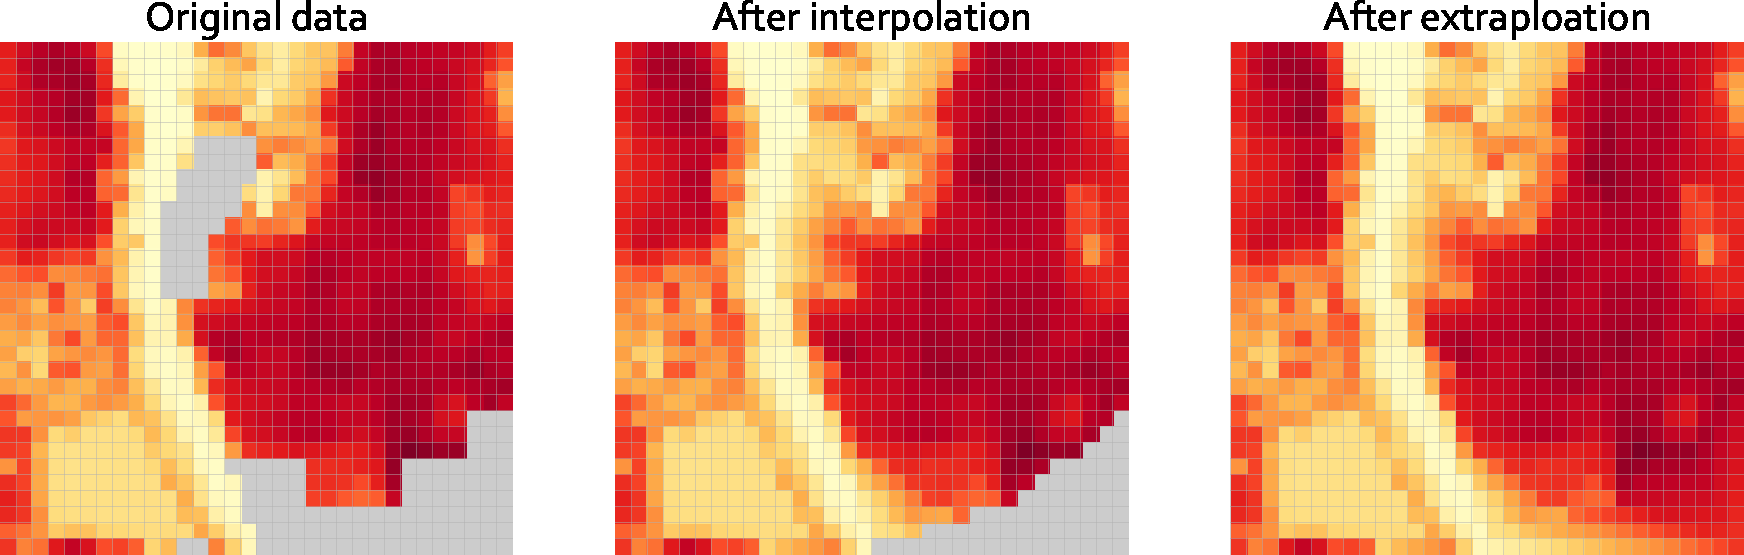
\includegraphics[width=\linewidth]{fig/report/cnn_data_prep.pdf}
    \caption{Handling of missing data for the CNN. The image shown is for a $32 \times 32$ cell section of mean day temperature for Portland at the 100m resolution.}
    \label{fig:cnn_missing_data}
\end{figure*}


\subsection{Model}

The model architecture is shown in Figure~\ref{fig:cnn_architecture}. It consists of multiple convolutional layers at both the input resolution and a 50\% downsampled resolution. Additionally, a skip connection concatenates the raw input data with one of final layers to reduce the depth between the input and output.

\begin{figure*}[h]
    \centering
    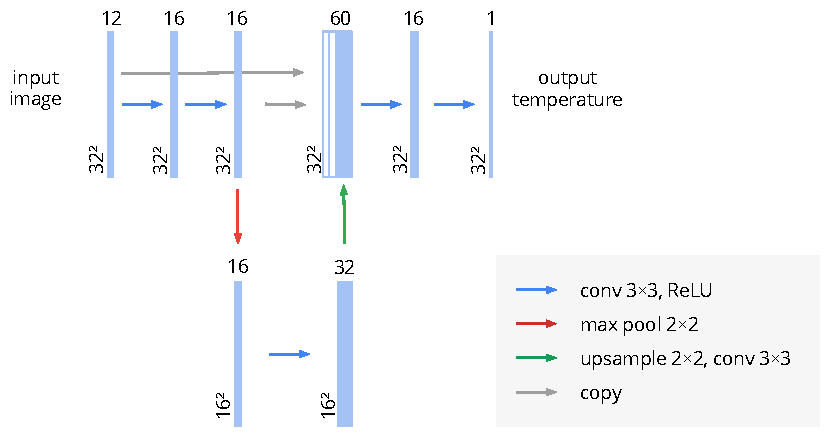
\includegraphics[width=\linewidth]{fig/report/cnn_architecture_cropped.pdf}
    \caption{CNN model architecture. Each layer shows the spatial dimensions (e.g., $32^2$) and the number of channels (e.g., 12). In the final {$32^2 \times 1$} layer, the ReLU layer is omitted.}
    \label{fig:cnn_architecture}
\end{figure*}

The size of the network is much smaller compared to the original U-Net in order to reduce overfitting due to our small dataset.

The final layer uses a linear activation function to enable regression. All other layers use ReLU activation, and dropout is applied after the contraction.

To prevent the CNN overfitting to the naively-imputed missing data, a masked loss function was used. The mean square error was greatly reduced for cells $i$ with missing data according to a mask $M$

\begin{align*}
    \mathrm{loss}_i &= M_i(y_i - \hat y _i) ^ 2\\
    M_i &= \begin{cases}
      0.01, & \text{if}\ y_i \mathrm{undefined} \\
      1, & \text{otherwise}
    \end{cases}
\end{align*}

This reduces the impact missing data has on the model weights, while leaving a small amount of gradient to avoid numerical issues with lack of convergence. The cells with missing data were excluded from any results presented.

The mask was also added to the input data as an additional channel.





\newpage
\section{City specific results}
\label{ss:city}
\begin{figure}[h]
    \centering
    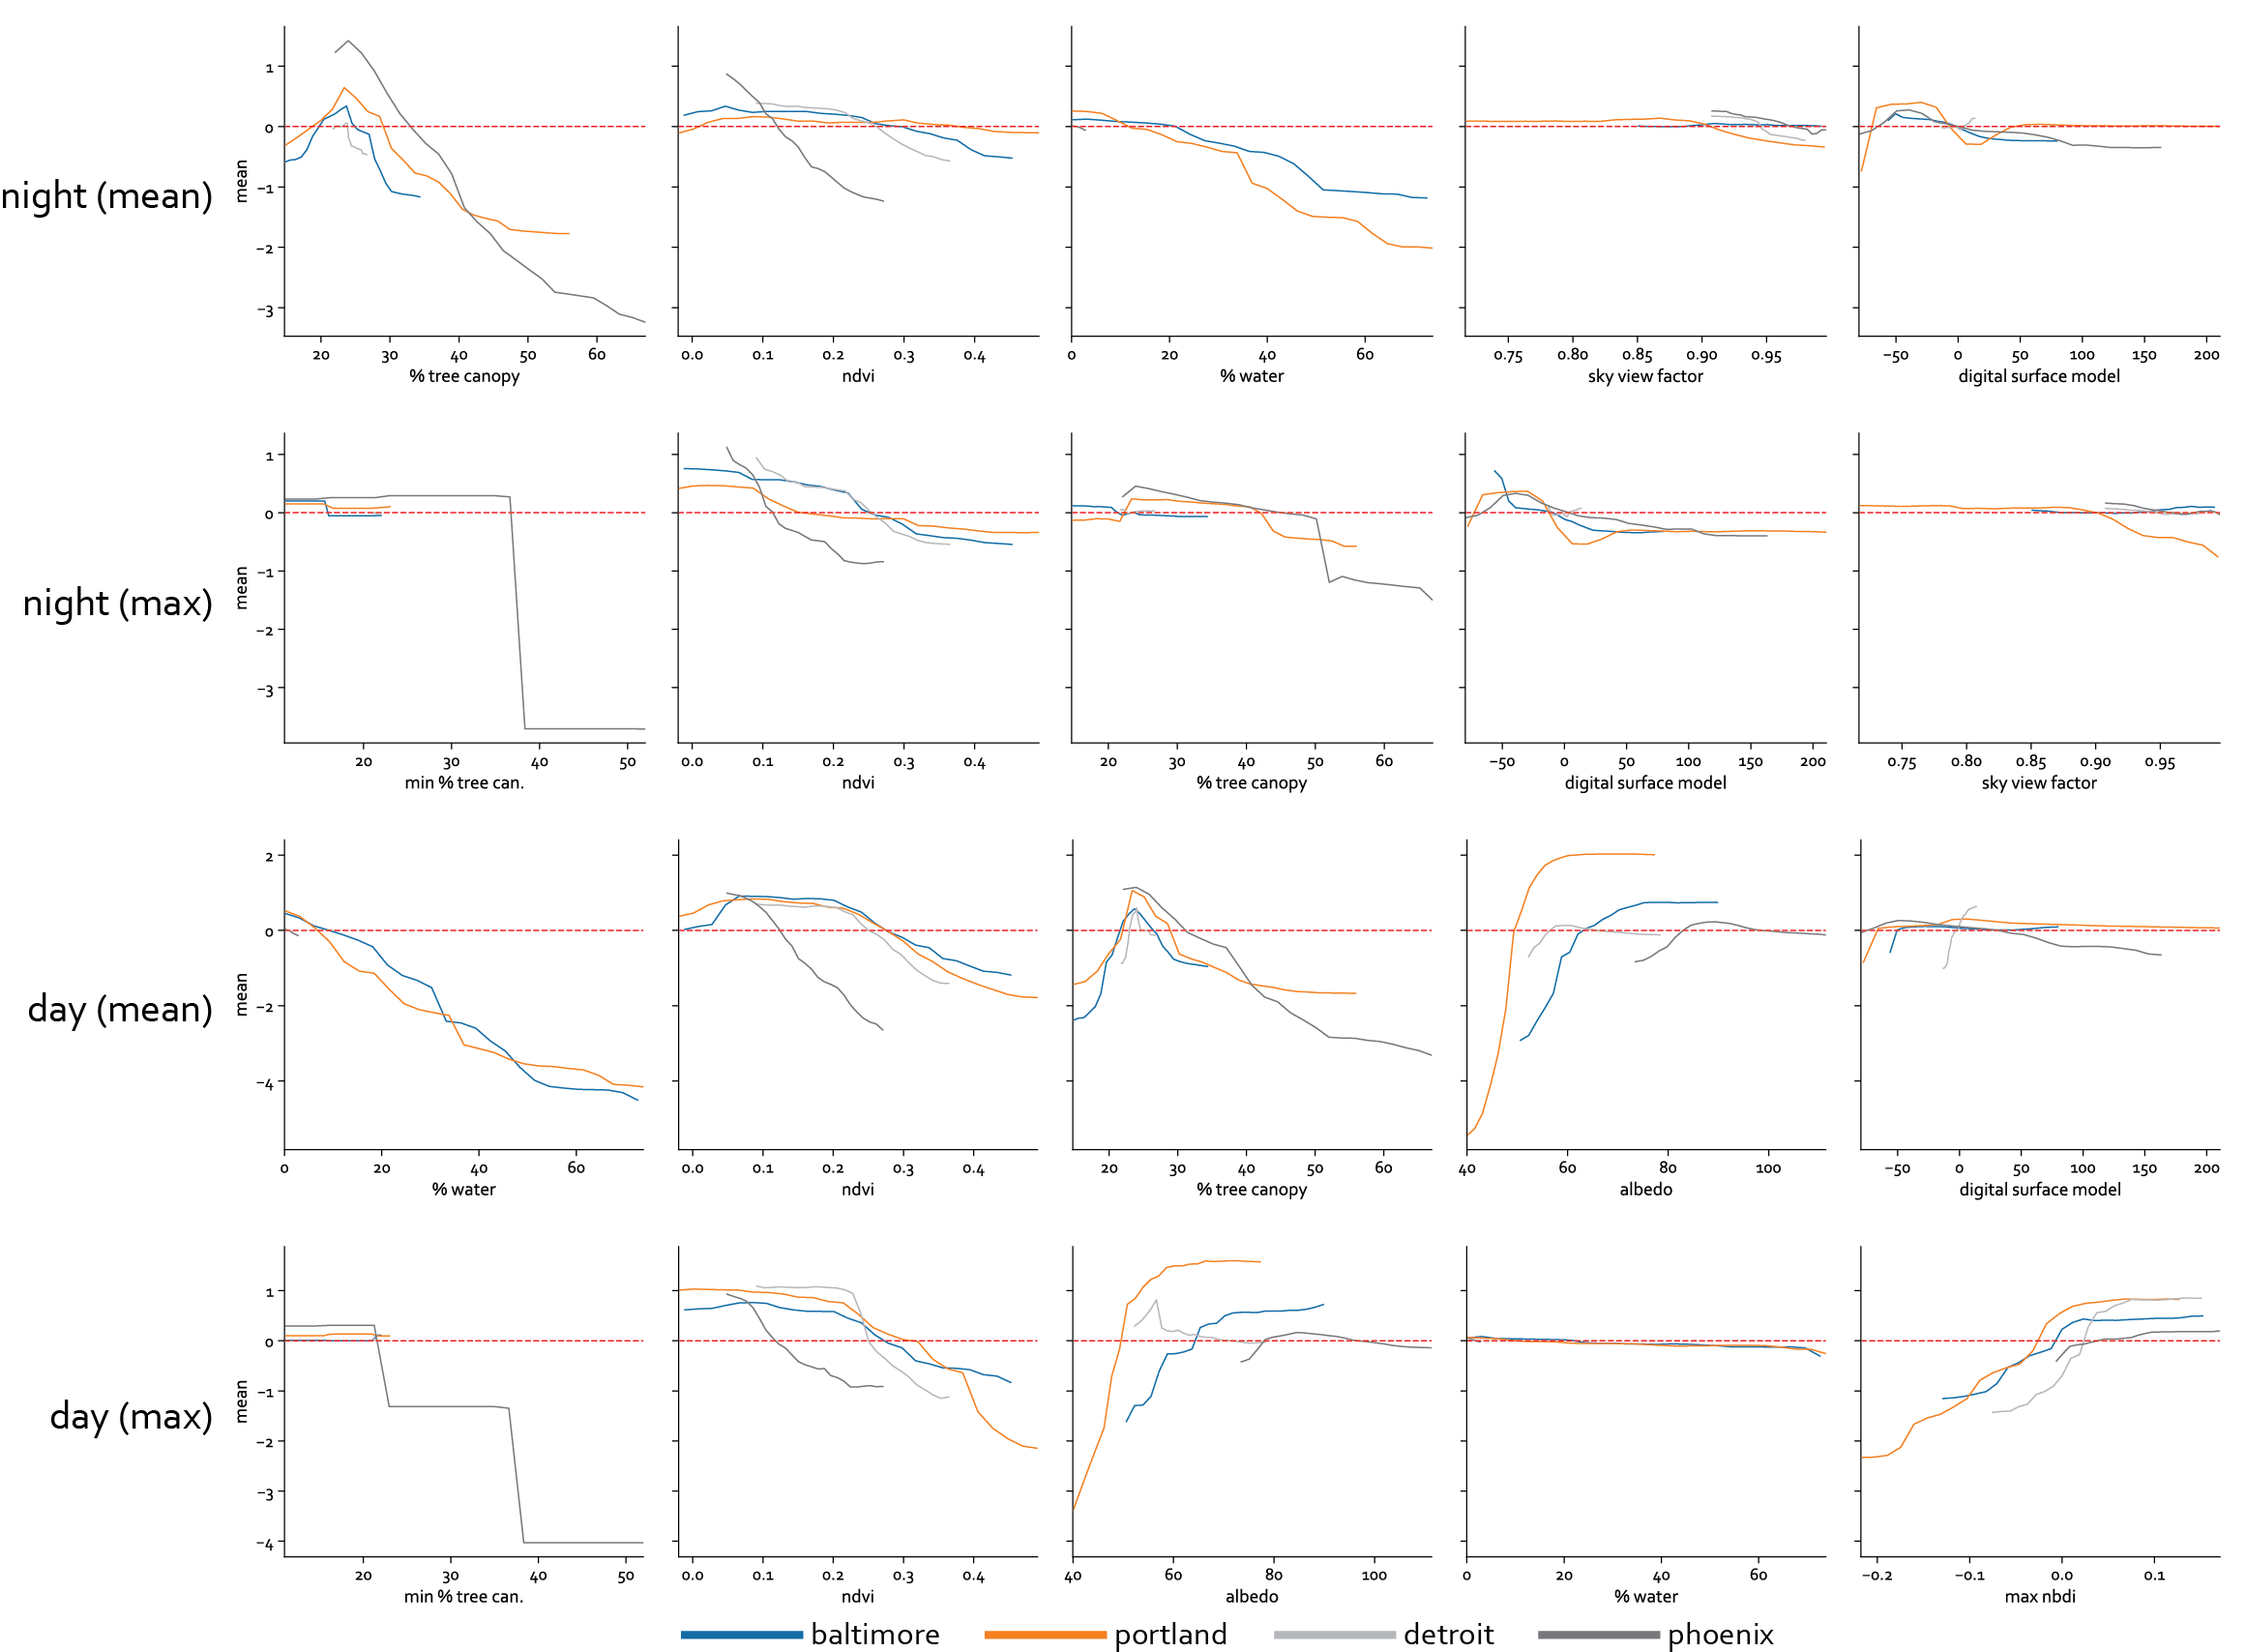
\includegraphics[width=\linewidth]{fig/report/pdp_cities_500.png}
    \caption[City specific partial dependence plots at the 500-meter resolution]{
    City specific partial dependence plots at the 500-meter resolution.
    The partial dependence plots for a random forest model trained on each city.
    This is to evaluate whether the influence of urban characteristics on LST is consistent between the cities.
    }
    \label{fig:cities_500}
\end{figure}

\begin{figure}[h]
    \centering
    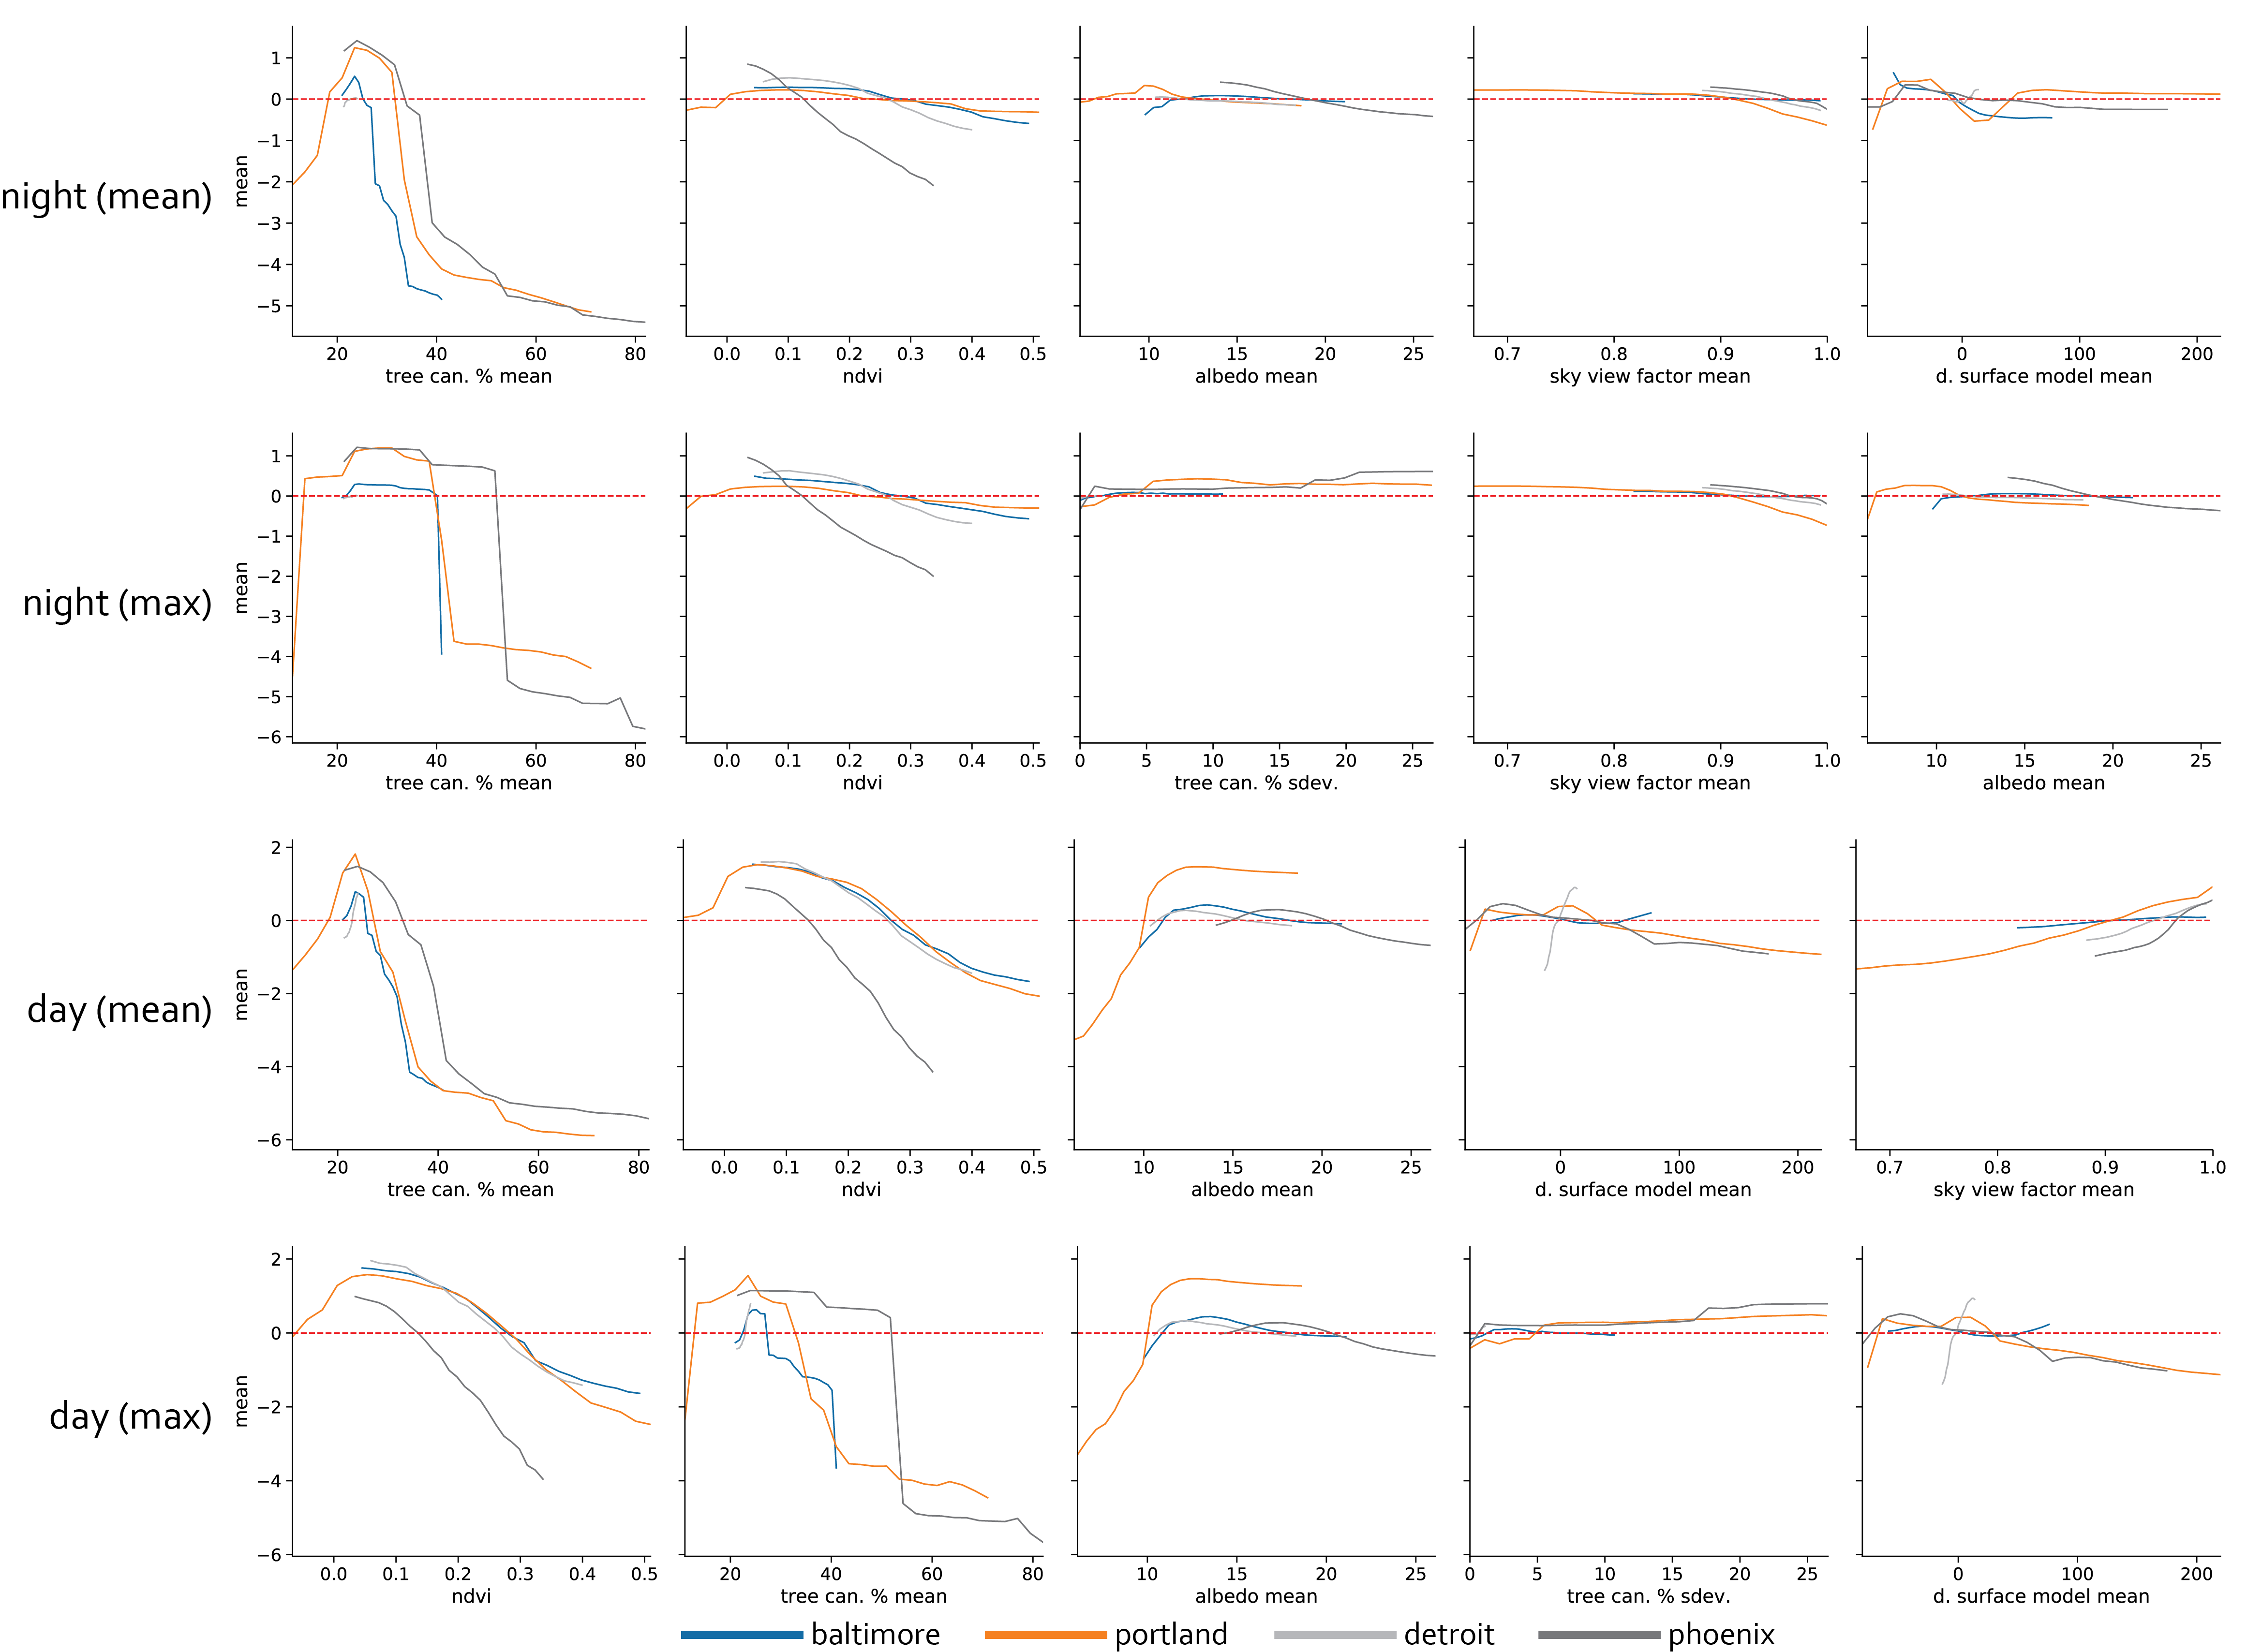
\includegraphics[width=\linewidth]{fig/report/pdp_cities_100.png}
    \caption[City specific partial dependence plots at the 100-meter resolution]{
    City specific partial dependence plots at the 100-meter resolution.
    These are partial dependence plots for a random forest model trained on each city.
    This is to evaluate whether the influence of urban characteristics on LST is consistent between the cities.
    }
    \label{fig:cities_100}
\end{figure}


\clearpage
\section{500-meter resolution results}
\label{ss:500_meter}
The figures presented in the main text, are replicated here based on data at a 500-meter resolution.

\begin{figure*}[h]
    \centering
    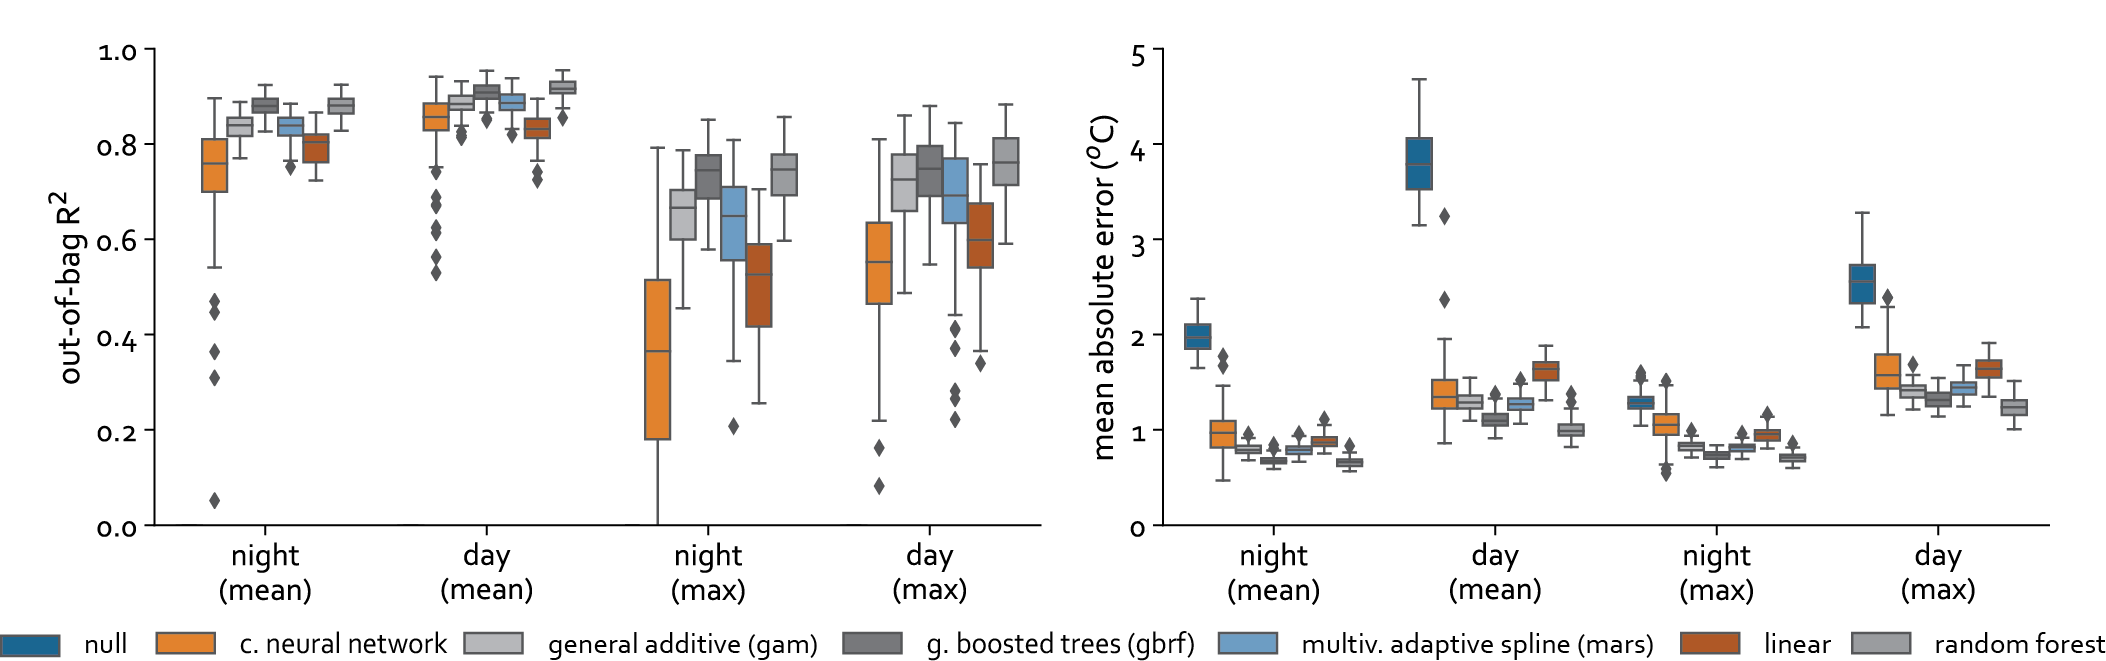
\includegraphics[width=\linewidth]{fig/report/holdout_500.png}
    \caption[Holdout cross-validation results at 500-meter resolution]{
    Holdout cross-validation results at 500-meter resolution. 
    The out-of-bag (OOB) R$^2$ and mean absolute error (MAE) of the models from a 500-fold holdout cross-validation. 
    The models were trained on 80\% of the data and tested on the unseen 20\%.
    When selecting data for the training and testing sets, spatial subsets were used to account for spatial similarities. 
    OOB R$^2$ can vary between $(-\infty, 1)$, where better models have a value near 1. 
    Good models have MAE near 0.
    }
    \label{fig:holdout_500}
\end{figure*}



\begin{figure*}[h]
    \begin{center}
    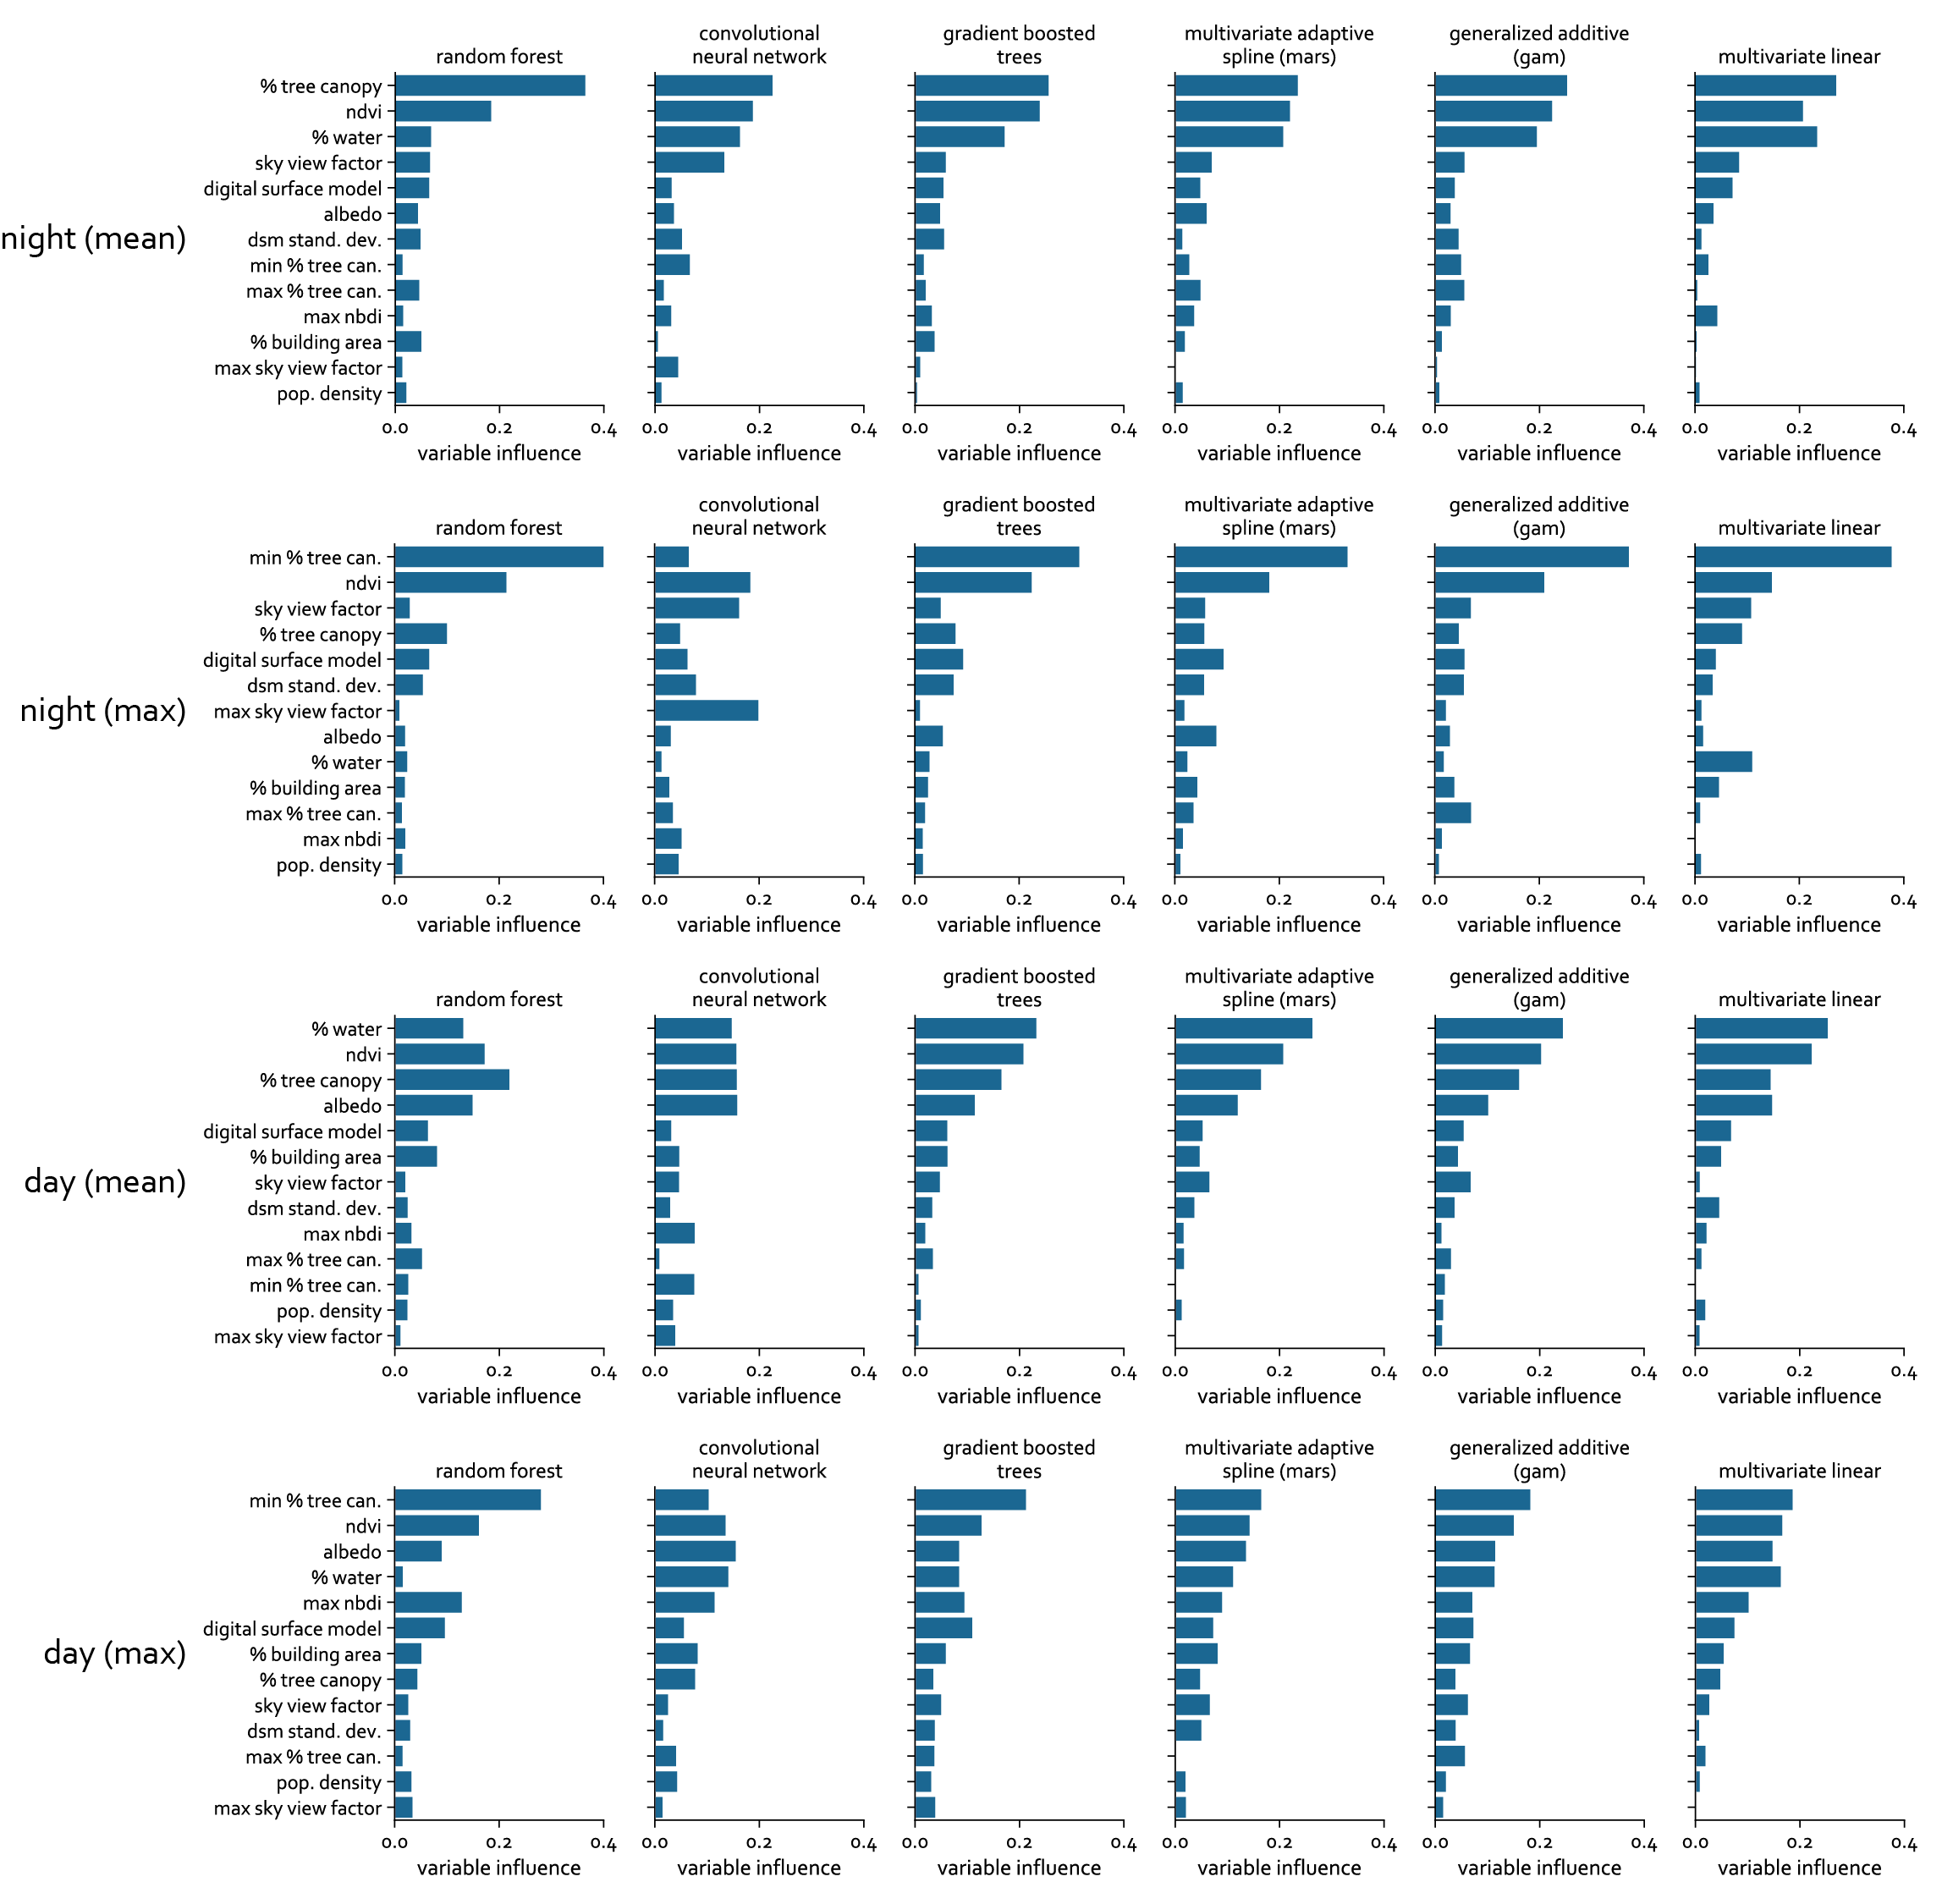
\includegraphics[width=\linewidth]{fig/report/importance_500.png}
    \caption[Variable influence on LST at 500-meter resolution]{
    Variable influence on LST at 500-meter resolution.
    The variable influence, measured by swing, shows the relative importance of each urban characteristic on land surface temperature.}
    \label{fig:importance_500}
    \end{center}
\end{figure*}


\begin{figure*}[h]
    \centering
    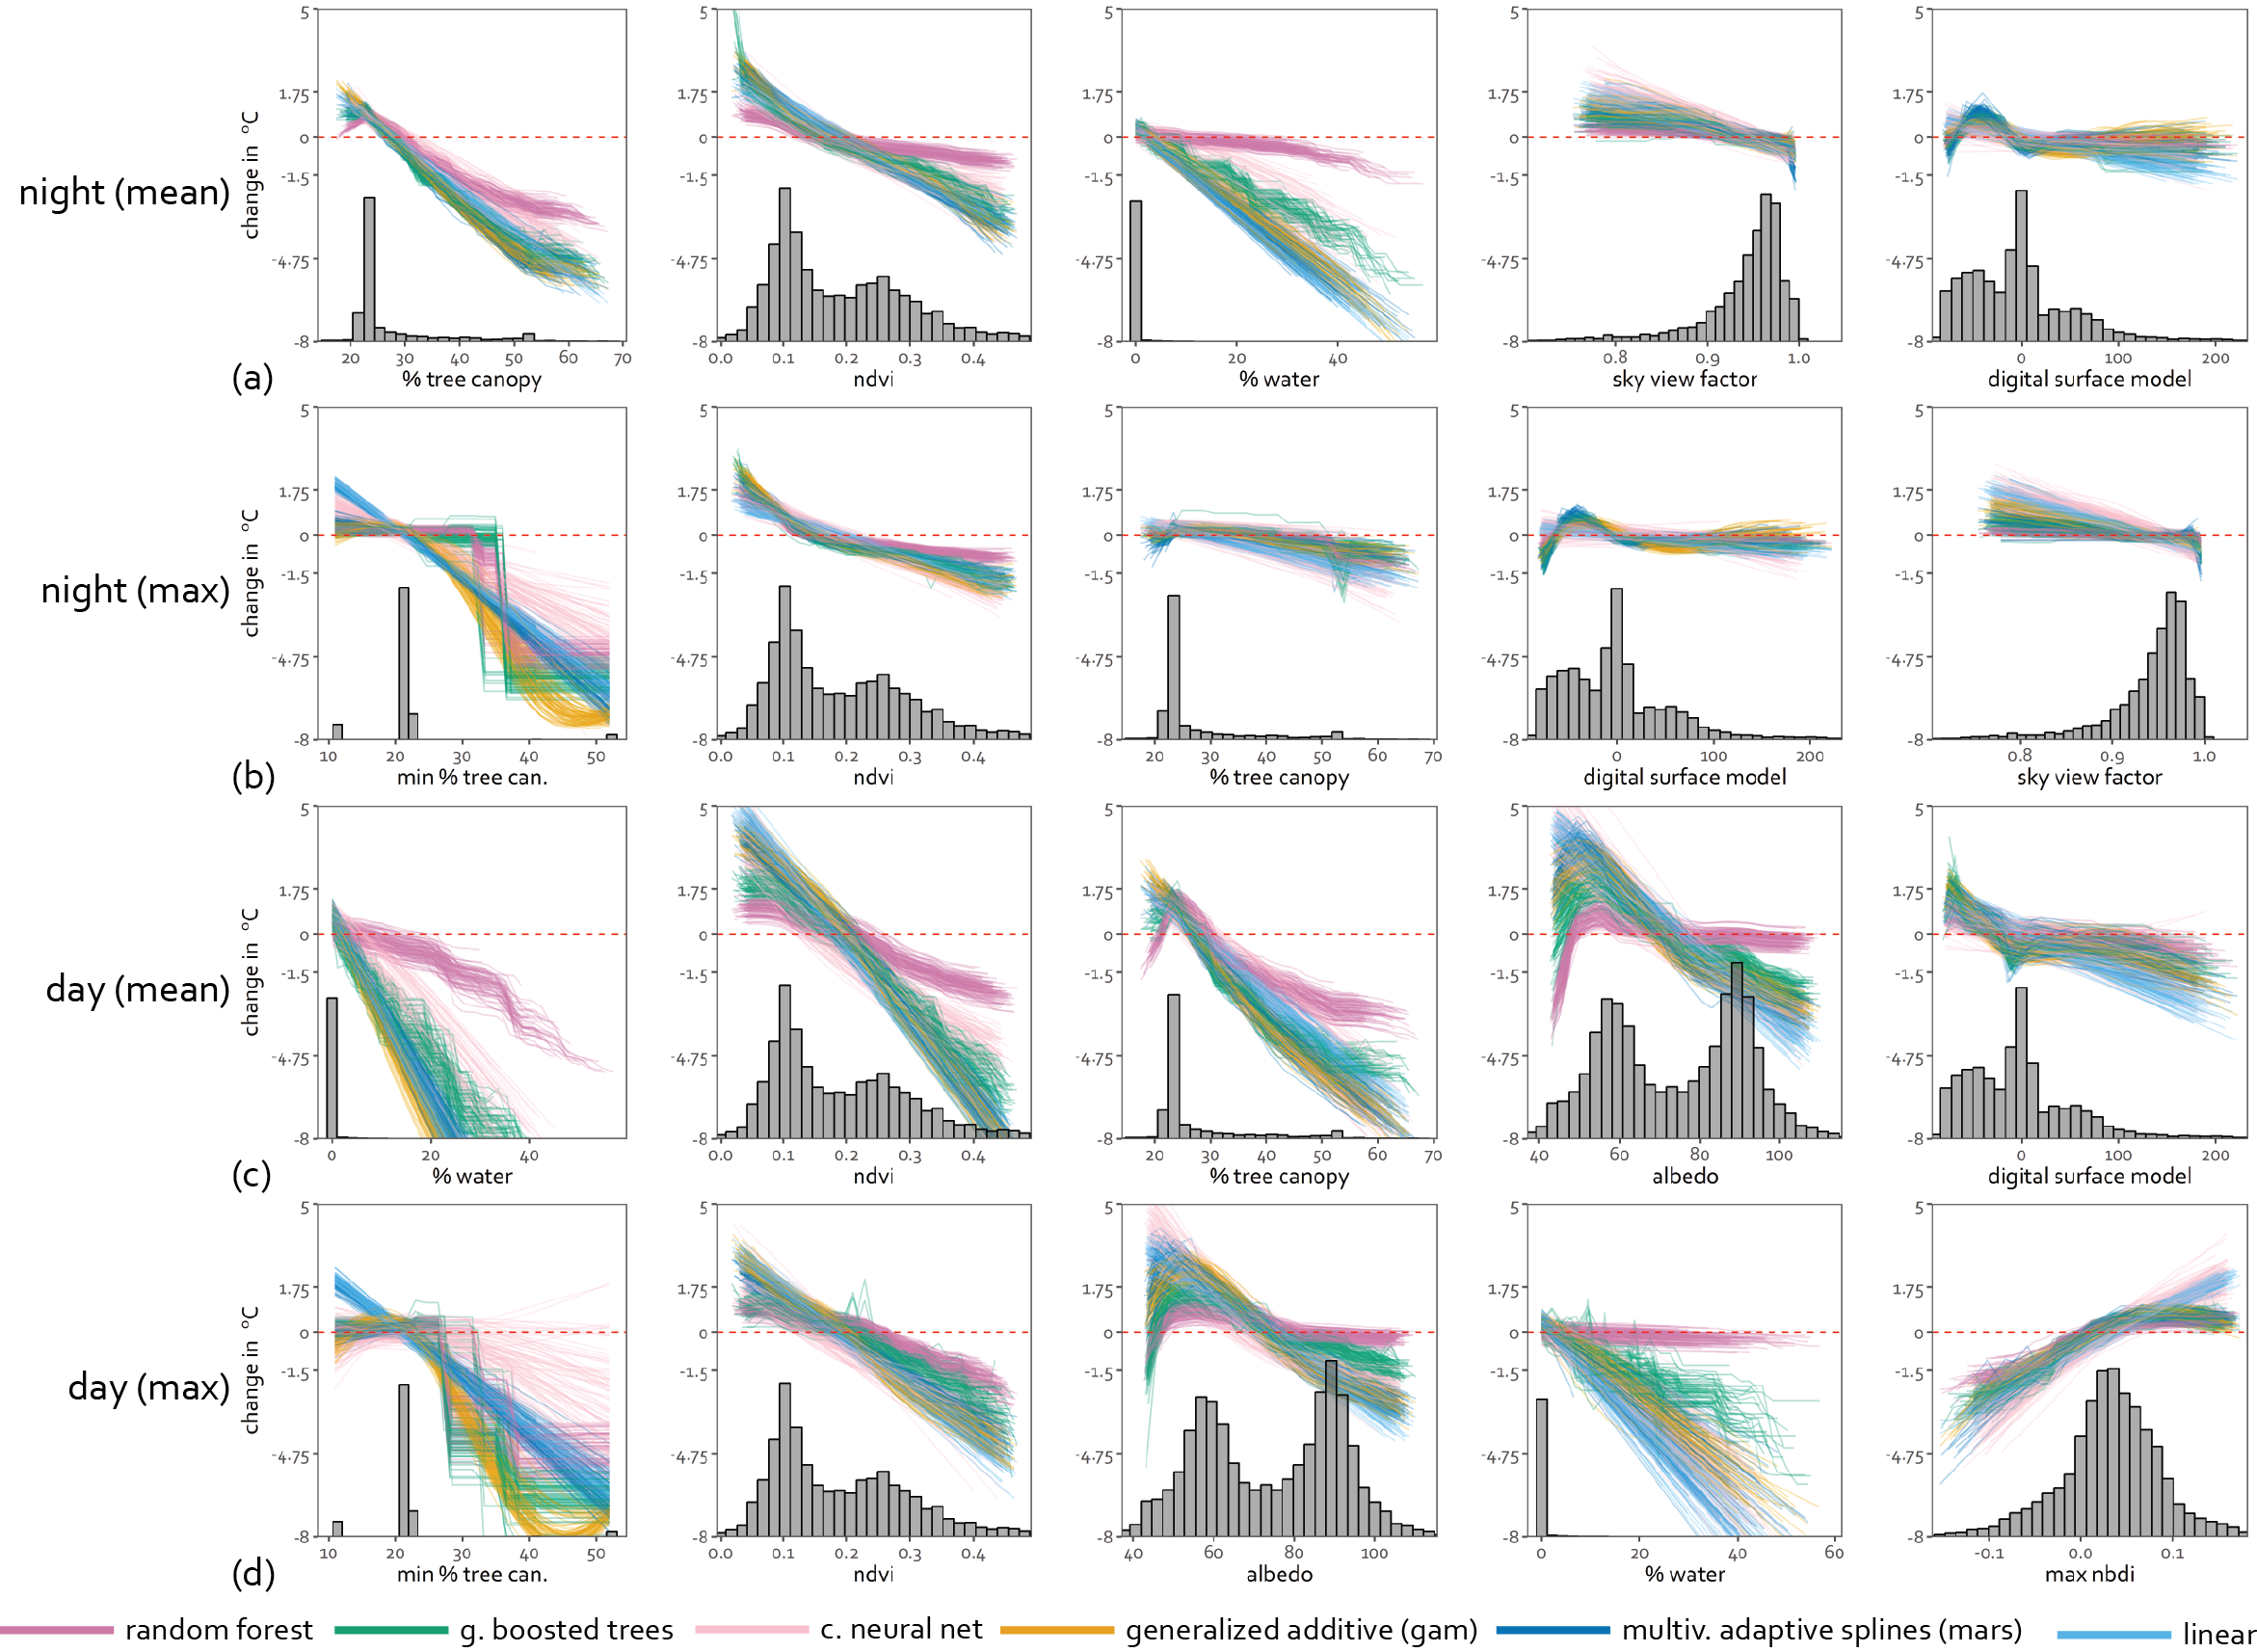
\includegraphics[width=\linewidth]{fig/report/pdp_500.png}
    \caption[Partial dependence plots for LST at 500-meter resolution]{
    Partial dependence plots for LST at 500-meter resolution.
    Partial dependence plots show how the land surface temperature ($^oC$, y axis) changes with each urban characteristic as the other variables are held at their average (mean) value. 
    The left hand side shows the effect each variable has on the (a) mean land surface temperature (LST) during the night, (b) maximum LST during the night, (c) mean LST during the day, (d) maximum LST during the day. 
    Each of the models are shown and this indicates the model uncertainty in the relationships.
    There are multiple lines for each model based on bootstrap samples of the data, which indicates the data uncertainty.
    The histograms on the $x$-axis shown the distribution of the observed data.
    }
    \label{fig:pdp_500}
\end{figure*}

\begin{figure}[h]
    \centering
    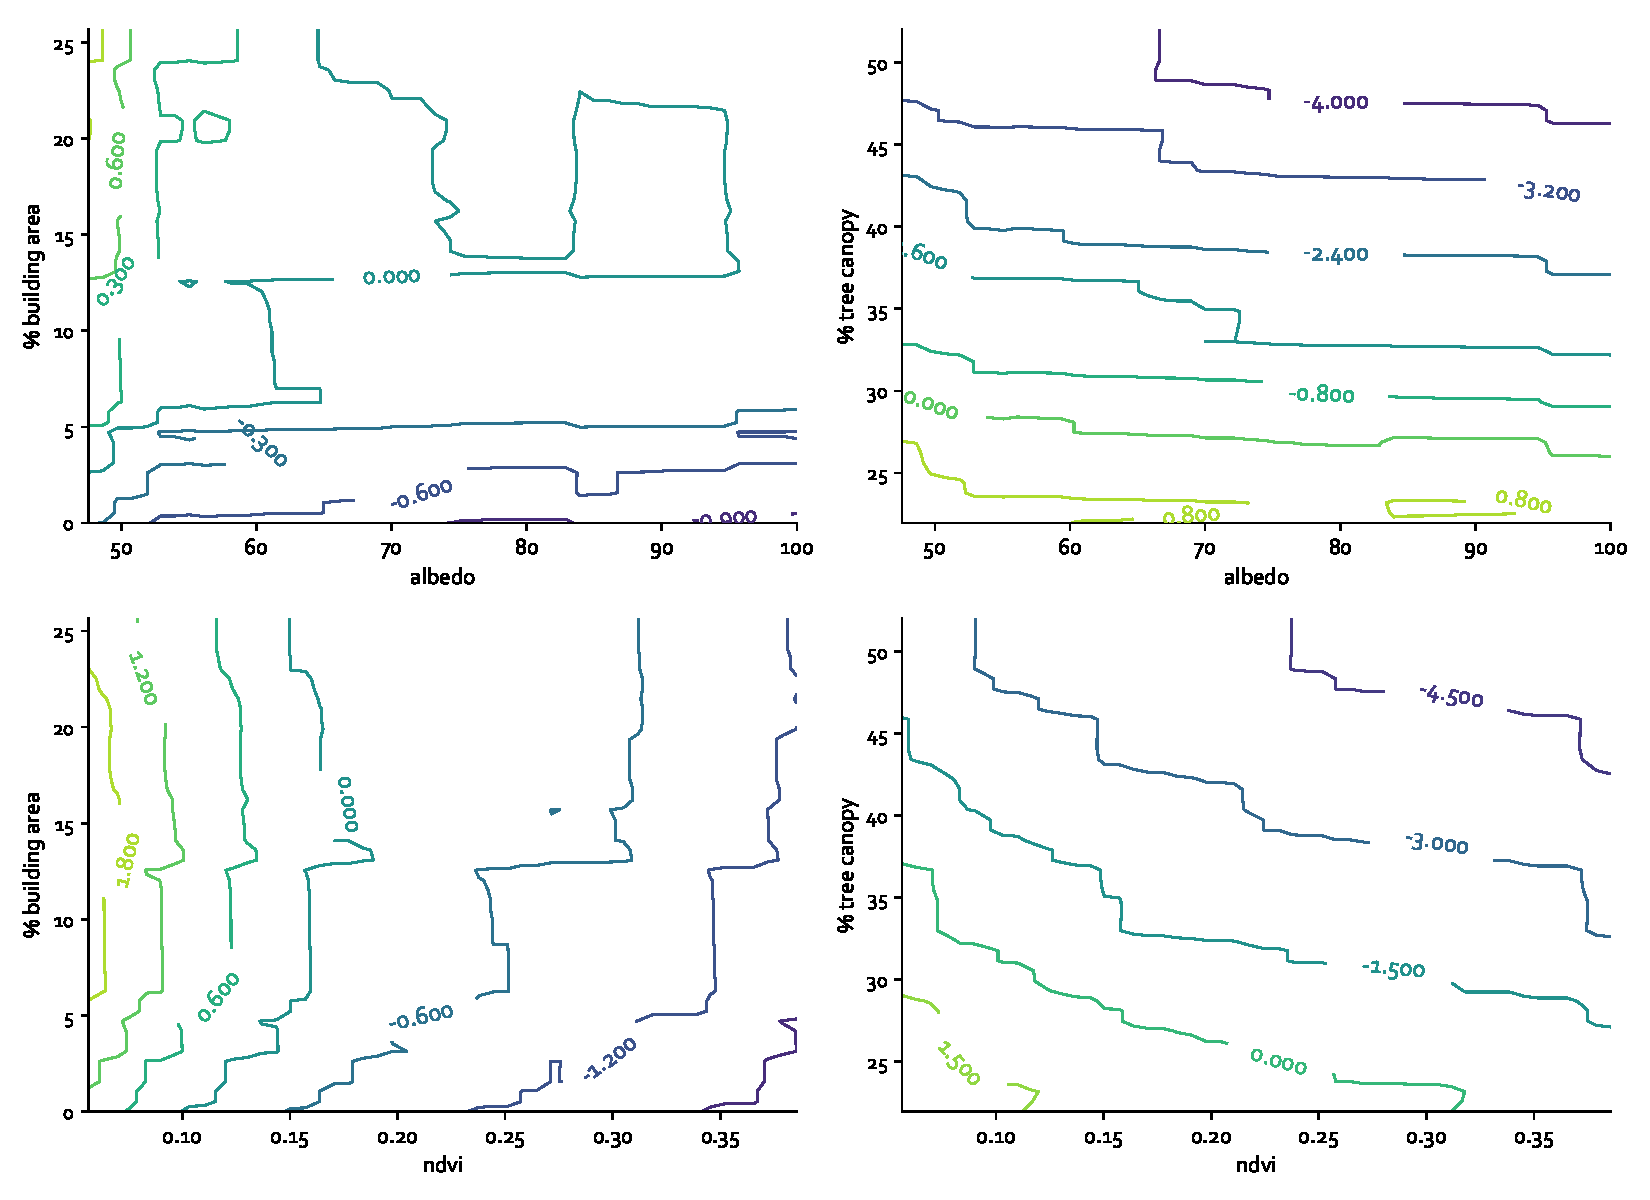
\includegraphics[width=\linewidth]{fig/report/pdp_2d_night_500.pdf}
    \caption[Partial dependence contour plots for LST at 500-meter resolution during the night]{
    Partial dependence contour plots for LST at 500-meter resolution during the night.
    These partial dependence contours show how the land surface temperature ($^oC$, y axis) changes with each variable as the other variables are held at their average value. The left hand side shows the effect each variable has on LST during the night, while the right hand side shows the effect during the day. This shows that trees coverage in the cell has the greatest influence on the temperature, and the greenness (NDVI) of that coverage matters during the day.
    }
    \label{fig:pdp_2dnight_500}
\end{figure}

\begin{figure}[h]
    \centering
    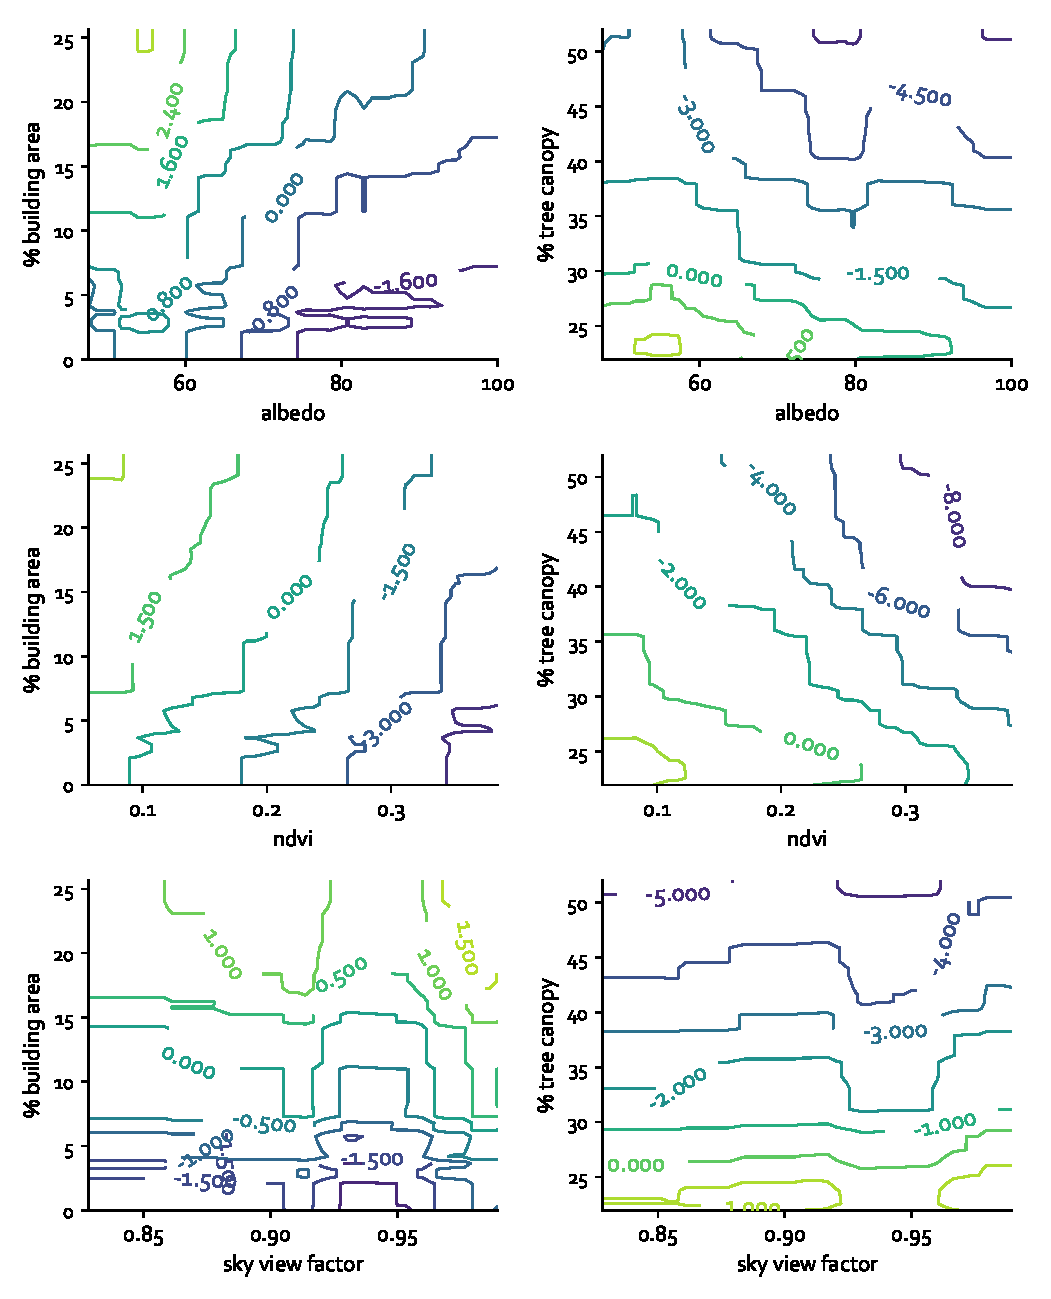
\includegraphics[width=\linewidth]{fig/report/pdp_2d_day_500.pdf}
    \caption[Partial dependence contour plots for LST at 500-meter resolution during the day]{
    Partial dependence contour plots for LST at 500-meter resolution during the day.
    These partial dependence contours show how the land surface temperature ($^oC$, y axis) changes with each variable as the other variables are held at their average value. The left hand side shows the effect each variable has on LST during the night, while the right hand side shows the effect during the day. This shows that trees coverage in the cell has the greatest influence on the temperature, and the greenness (NDVI) of that coverage matters during the day.
    }
    \label{fig:pdp_2dday_500}
\end{figure}


\clearpage
\section{Additional figures}
\begin{figure*}[h]
    \centering
    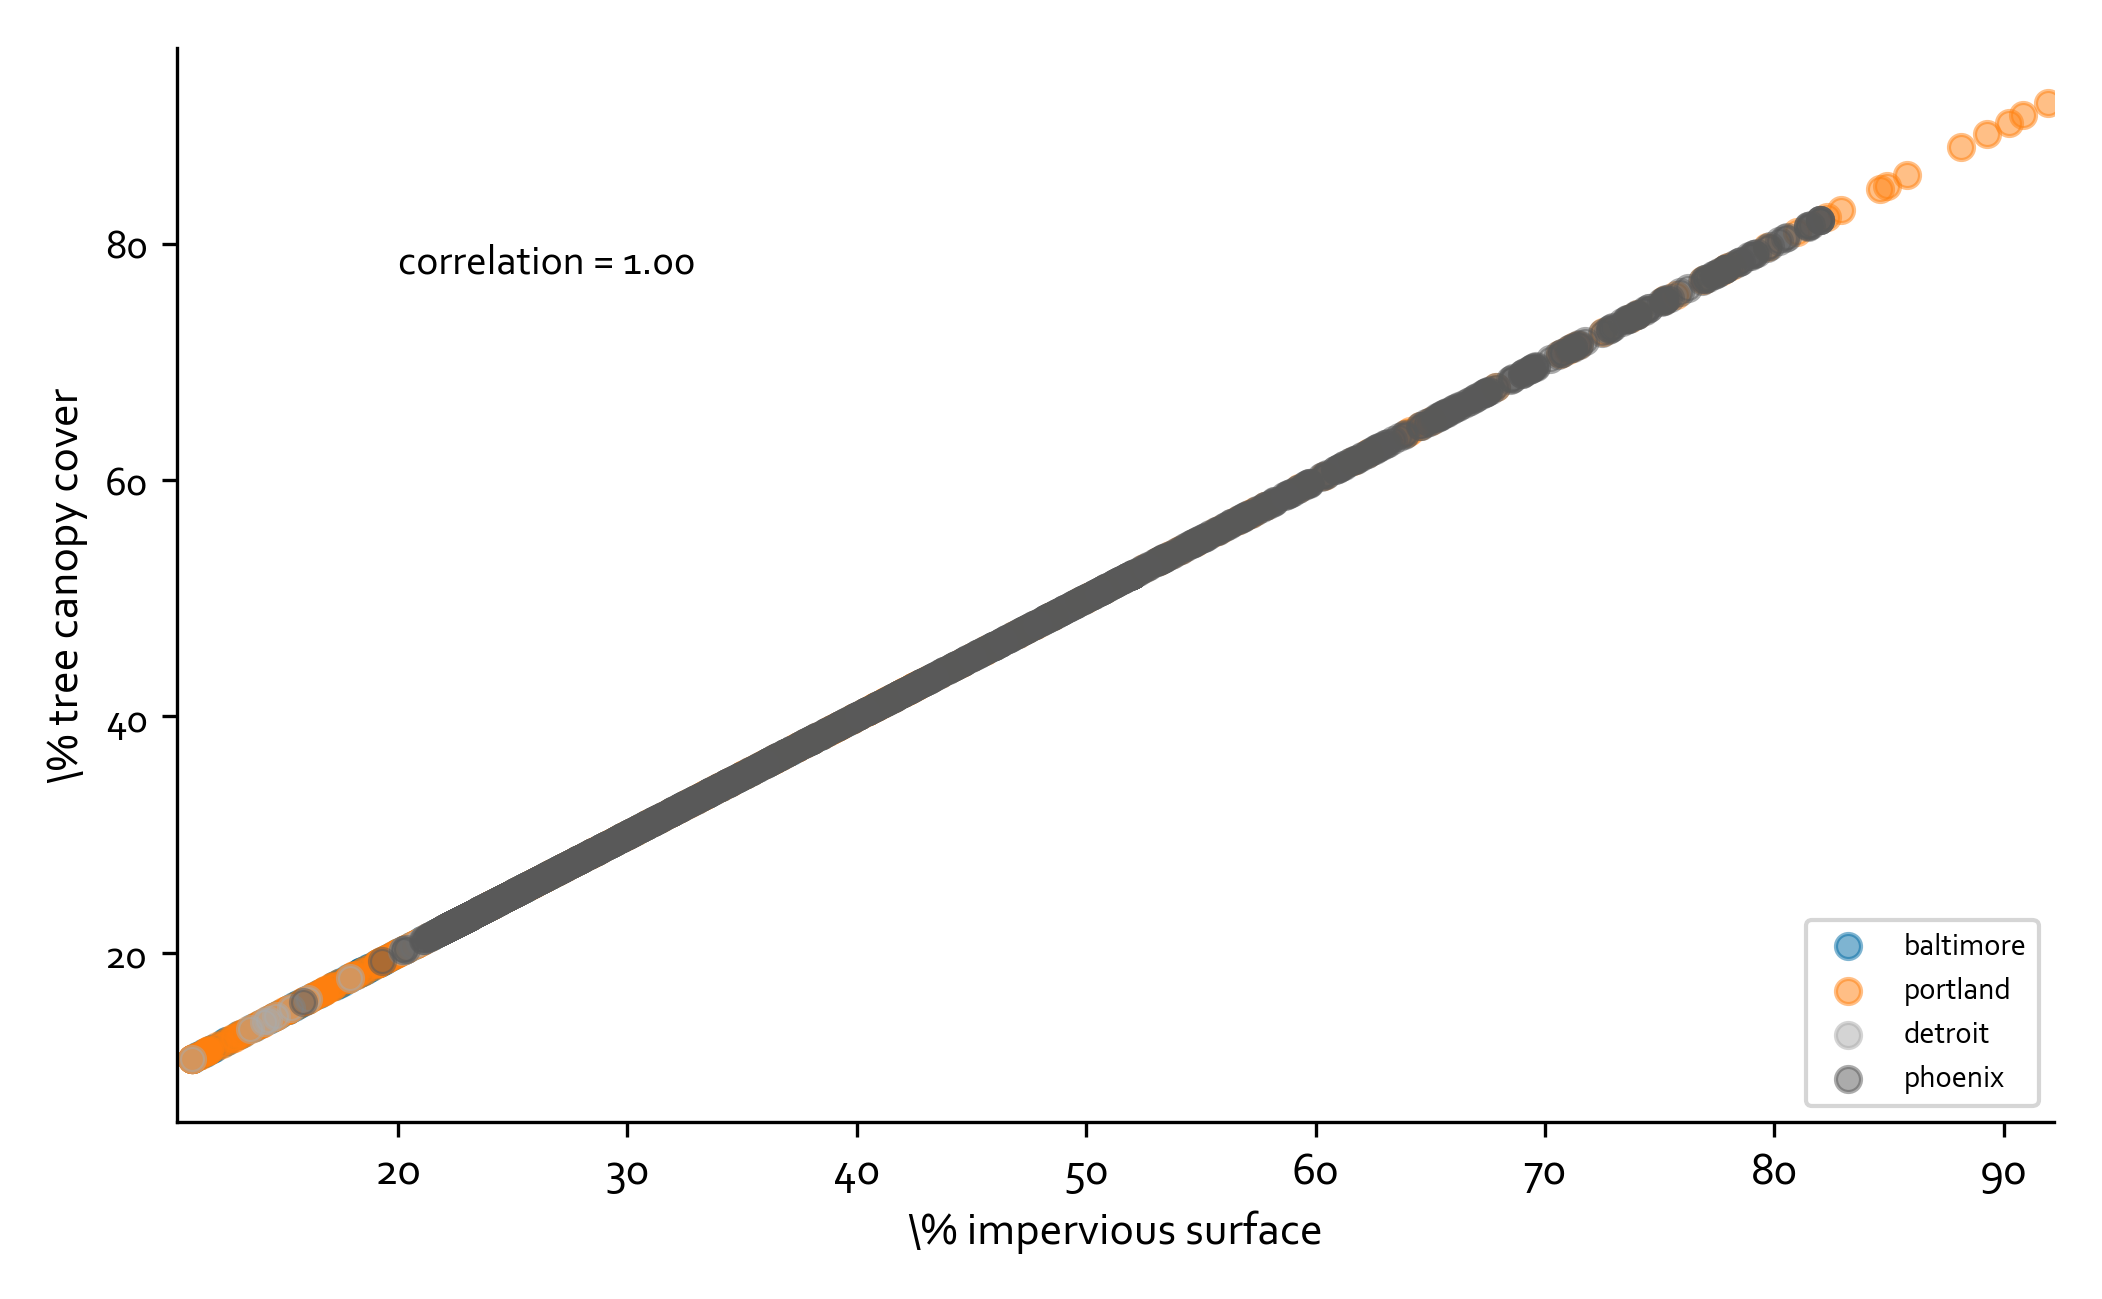
\includegraphics[width=\linewidth]{fig/report/imp_v_tree_500.png}
    \caption{
    Percentage tree canopy cover and impervious surface are 100\% correlated.
    }
    \label{fig:imp_tree}
\end{figure*}


\end{document}
